
\chapter{The reconstruction for the water-phase}
\label{chap:recon}
After carefully calibrating the PMTs, we can obtain the number of photons hitting the PMT and their arrival times for each event. Based on these information, we will use statistical methods to infer information such as the position, energy, and direction of the physical events that produced these photons.
In the field of Cherenkov reconstruction, the Super-Kamiokande~(SK) experiment is the most worthy of reference. SK stands as the world's largest pure water Cherenkov detector, housing \SI{50}{kilotons} of ultrapure water~\cite{SK}. Building upon the liquid scintillator-Cherenkov combined track reconstruction technique developed for the MiniBooNE experiment~\cite{minibone}, SK collaboration has advanced a likelihood-based reconstruction method, utilizing PMT charge and time information~\cite{SKfiTQun}, named as fiTQun. For JUNO water-phase, we have implemented targeted improvements to the fiTQun and extended its application to low-energy event reconstruction at the \si{MeV} scale.

\section{The Likelihood function}
\label{sec:recon}
FiTQun simultaneously determines particle types, vertex positions, momentums, event times.
In JUNO water-phase, we just need to determine the vertex position, momentums and event times.
The likelihood function of fiTQun is defined as:
\begin{equation}
	\begin{aligned}
		\log \mathcal{L}(\boldsymbol{x};{q},{t}) = & \sum_{j \in \{q=0\}} \log P_j \bigl( q=0\bigm| \mu_j \bigr)                                      \\
		                                           & + \sum_{i \in \{q>0\}} \log \bigl( f_{\mathrm{q}}\bigl( q_i \bigm| \mu_i \bigr) \bigr)           \\
		                                           & + \sum_{i \in \{q>0\}} \log \bigl( f_{\mathrm{t}} \bigl( t_i \bigm| \boldsymbol{x} \bigr) \bigr)
	\end{aligned}
\end{equation}
\begin{itemize}
	\item $\boldsymbol{x} = (t_0, x, y, z, p_x, p_y, p_z)$: Event vertex containing time $t_0$, position $(x,y,z)$, and momentum $(p_x,p_y,p_z)$.
	\item $\mu_i(\boldsymbol{x})$: Expected PEs at the $i$-th PMT, computed from the vertex $\boldsymbol{x}$.
	\item $q_i$: Charge observed at the $i$-th PMT, $\{q\}$ is the sequence of $q_i$, when $q_i=0$, the PMT is unhitted.
	\item $t_i$: Hit time of the $i$-th PMT, $\{t\}$ is the sequence of $t_i$.
\end{itemize}

The first term is the unhit likelihood, which is the probability of no hit in the PMT. The second term is the hit likelihood, which is the probability of detecting hits in the PMT. The third term is the time likelihood, which is the probability of detecting a hit at a certain time.

Since in the operation of the detector, only TQ information (time and charge) is recorded for low-energy events, waveform information is unavailable. At the same time only the first hit time can be obtained. Therefore, it is necessary to reformulate the likelihood to adopt a first-hit-time-based reconstruction approach. Xuewei Liu~et.al developed a first-principles-based reconstruction method using time-charge information or time-PE information in liquid scintillator detectors~\cite{Liu:2024cxo}. We adapt their methodology to reformulate the likelihood function for JUNO water-phase. In low-energy events, where each PMT typically detects only few photon, the number of hits can be directly approximated as NPE~($N_{PE}$). We can reformulate the likelihood function as Eq.~\eqref{eq:likelihood}:
\begin{equation}
	\begin{aligned}
		\log \mathcal{L}(\boldsymbol{x};{q},{t})= & \sum_{j \in \{q=0\}}\log P_j \bigl( q=0\bigm| \mu_j \bigr)+                                                                                                                        \\
		                                          & \sum_{i \in \{q>0\}} \log \bigl( f_{\mathrm{q}}\bigl( 0 \bigm| \mu_{i,\underline{t}}^{t_i} \bigr)f_{\mathrm{t}}(t_i)f_{\mathrm{q}}(N_{PE,i}-1|\mu_{i,t_{i}}^{\overline{t}}) \bigr)
	\end{aligned}
	\label{eq:likelihood}
\end{equation}

In this case, we define the data taking as $[\underline{t} ,\overline{t} ]$, and the first hit time of the $i$-th PMT as $t_{i}$, $\mu_{i,\underline{t}}^{t_i}$ is the expected PEs in [$\underline{T}$,${T_i}$], same as $\mu_{i,t_{i}}^{\overline{t}}$.

\section{Response of the water-phase dector}
To compute the likelihood, we need to predict how many photons each PMT will detect when given a vertex. The more accurate the predictions are, the better the reconstruction performances. Therefore, we need a comprehensive understanding of the detector response and develop accurate models for it.
It naturally comes to mind that when a charged particle enters water, emits Cherenkov photons, and triggers the PMT, this process can be divided into two parts. One pertains to how Cherenkov light is emitted, while the other concerns how the Cherenkov photons propagate and are detected.

\subsection{The Cherenkov emission profile}
When a charged particle travels through a medium at a speed exceeding that of light, it emits Cherenkov photons within a specific solid angle range. The phenomenon arises from local polarization occurring along the charged particle's trajectory: when polarized molecules return to their ground state, they emit electromagnetic radiation. When the refractive index of the medium is $n$, and the speed of light in vacuum is $c_0$, the condition of particle speed~$v_p$ for Cherenkov emmision is $\beta=v_p/c_0>1/n$. When in pure water, whose refractive index is $n_w=1.333$, and the paitical is electron~($m_0=\SI{0.511}{MeV}$), the energy threthold is $E_{th}=m_0\times(\sqrt{1-1/n_w^2}-1)=\SI{0.262}{MeV}$. That means, only when the energy of electron is larger than \SI{0.262}{MeV}, the Cherenkov photons will emit.

The direction of Cherenkov photons can be discribed as: $\cos\theta=\frac{1}{\beta n_w}$ as Fig~\ref{Fig:Cherenkov_emmision} shown.

\begin{figure}
	\begin{center}
		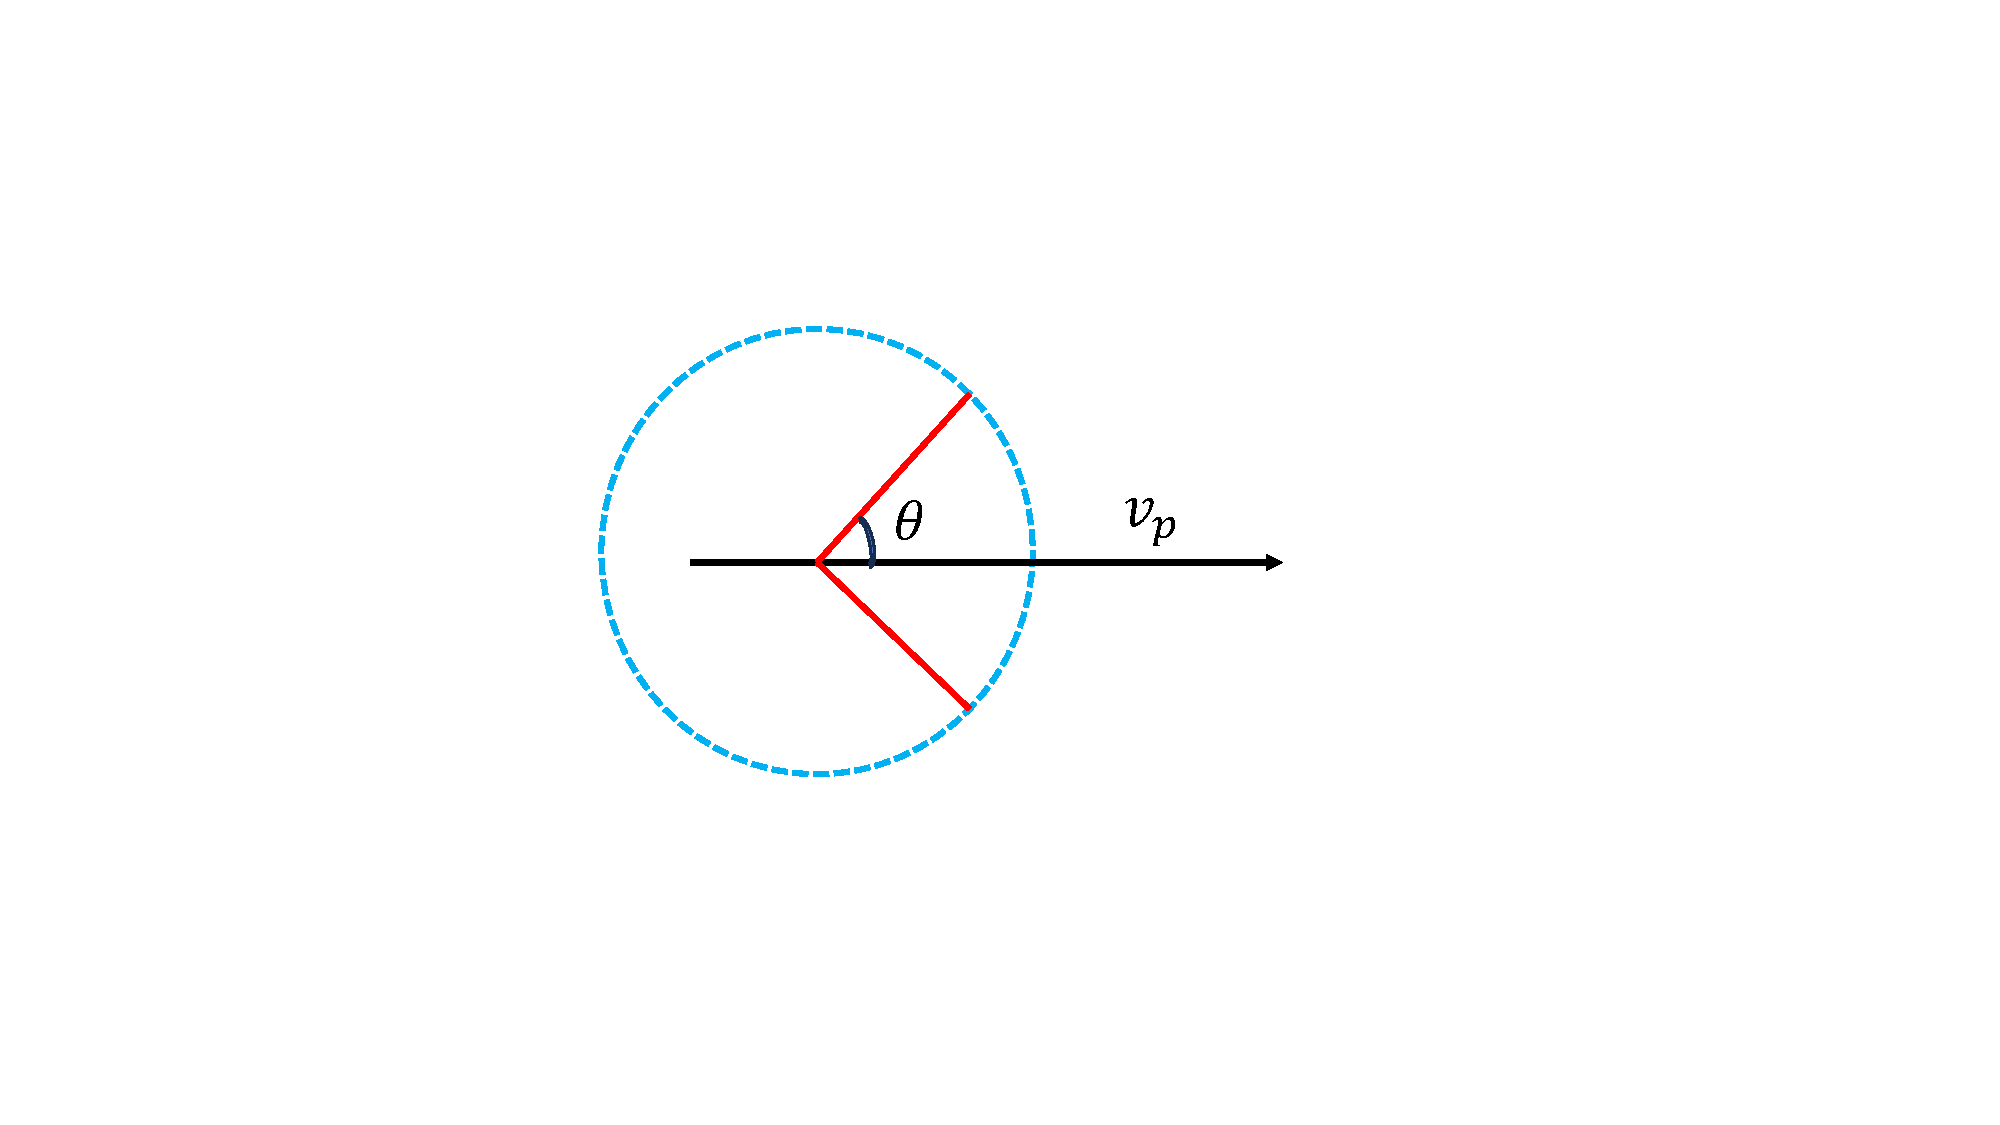
\includegraphics[height=6cm]{reconstruction/cherenkov_emission.pdf}
	\end{center}
	\caption{The direction of Cherenkov photons. $\theta$ is the angle between the photon emission direction and the direction of particle motion.}
	\label{Fig:Cherenkov_emmision}
\end{figure}

When in water, $\cos\theta\approxeq0.75$. We can use simulation to get the emmision profile of Cherenkov photons. Also, we consider the light yield of Cherenkov by simulating electron with momentum from \SI{2}{MeV} to \SI{30}{MeV}. Our simulation is based on JUNO software~(JUNOsw)~\cite{junosw}, and the version is J24.2.1. We simulated electrons with momenta ranging from 2 to \SI{50}{MeV}, uniformly distributed within the detector, while their emission directions were randomly oriented.

We extended Dou Wei's angular coordinate definition method for liquid scintillator detectors~\cite{Dou:2022} to Cherenkov radiation detection by incorporating momentum direction degrees of freedom, resulting in the coordinate system illustrated in the figure.

\begin{figure}
	\begin{center}
		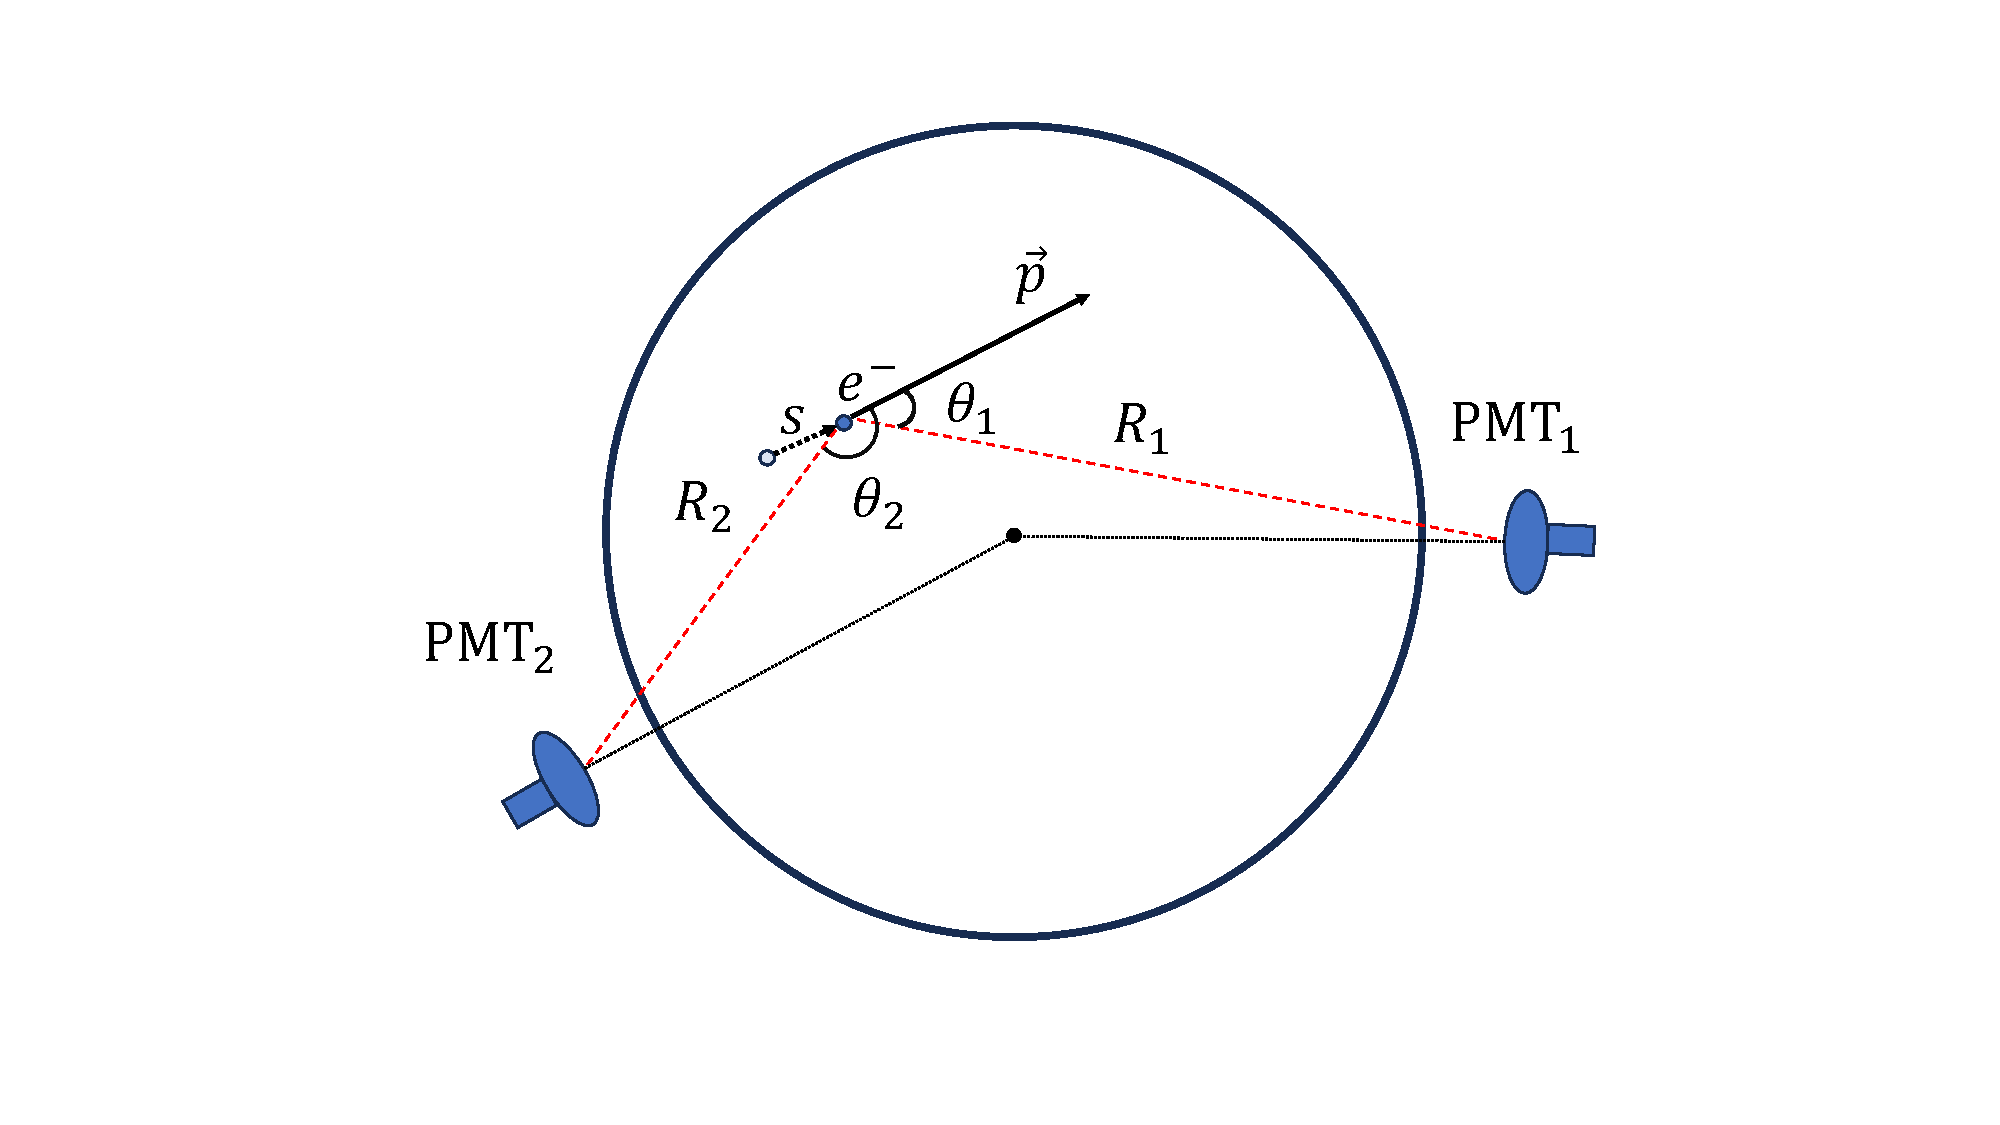
\includegraphics[height=6cm]{reconstruction/zuobiao.pdf}
	\end{center}
	\caption{Coordinate system definition: $\theta$ is the angle of the emission direction of Cherenkov photon and the incident direction of the electron, $s$ is the distance from the position where the particle emits light to its initial position. $R$ is the distance of PMT to the position of electron.}
	\label{Fig:Coordinate}
\end{figure}

In this simulation, we recorded the angles between the emission directions of all Cherenkov photons and the incident direction of the electron, and we do not care the photons are detected or not. Simultaneously, a crucial parameter is the distance between the photon generation point and the origin position of the charged particle.
\begin{itemize}
	\item From Fig~\ref{fig:thetaemmision}, most photons are emitted along the Cherenkov angle~($\cos\theta=0.75$), while a minority exhibit significant angular deviations from the electron's direction. When calculating the emission angle distribution, it must be analyzed separately for different particle energies rather than applying a single angular distribution to electrons of all energies.
	\item From Fig~\ref{fig:semmision}, as the particle moves, Cherenkov photons emitted along the initial segment of its trajectory exhibit a uniform distribution. When the particle's velocity significantly decreases, photon emission drops markedly, with the vast majority of photons being emitted within the first half of the trajectory.
	\item From Fig~\ref{fig:tsemmision}, after traveling some distance, the probability of photons deviating from the Cherenkov angle gradually increases due to multiple scattering. As illustrated in the figure, when electrons undergo multiple scattering, their direction changes significantly, as Fig~\ref{fig:multipleScattering} shown. However, when calculating the Cherenkov emission angle, we still use the initial incident direction, thereby producing photons emitted at angles far from the ideal Cherenkov angle.
	\item In this case, we get the Cherenkov emmision profile~($g(p,s,\theta)$) which describes the proportion of Cherenkov photons emitted at specific locations and directions along the trajectory of a charged particle with a given energy, relative to the total number of emitted photons. For the convenience of research, we use momentum~($p$) instead of energy~($E$).
\end{itemize}

\begin{figure}[h]
	\centering
	\begin{subfigure}{0.45\textwidth}
		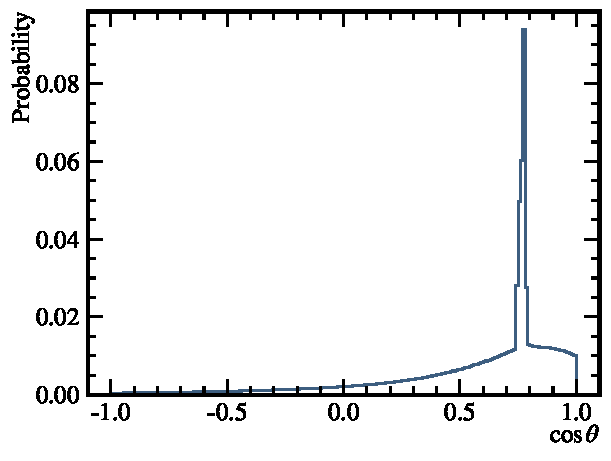
\includegraphics[page=1,width=\textwidth]{reconstruction/emmisionProfile/2.pdf}
		\caption{\SI{2}{MeV} electron}
		\label{fig:theta2mev}
	\end{subfigure}
	\hfill
	\begin{subfigure}{0.45\textwidth}
		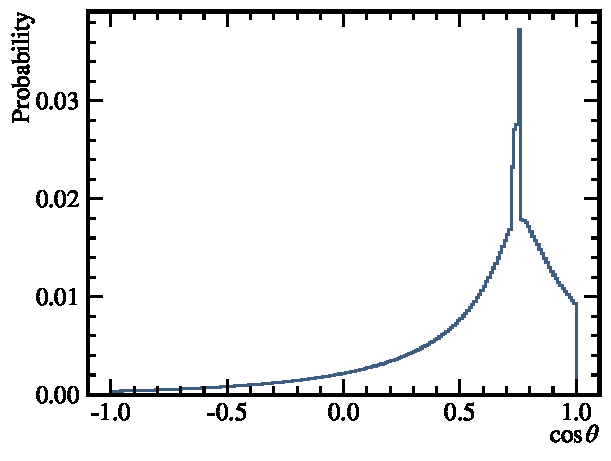
\includegraphics[page=1,width=\textwidth]{reconstruction/emmisionProfile/5.pdf}
		\caption{\SI{5}{MeV} electron}
		\label{fig:theta5mev}
	\end{subfigure}

	\vspace{\baselineskip}

	\begin{subfigure}{0.45\textwidth}
		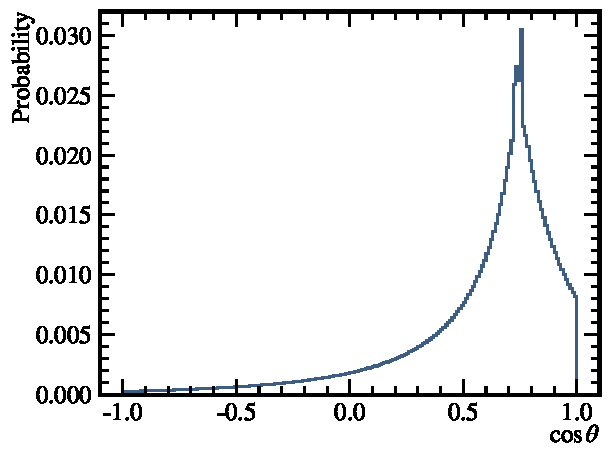
\includegraphics[page=1,width=\textwidth]{reconstruction/emmisionProfile/10.pdf}
		\caption{\SI{10}{MeV} electron}
		\label{fig:theta10mev}
	\end{subfigure}
	\hfill
	\begin{subfigure}{0.45\textwidth}
		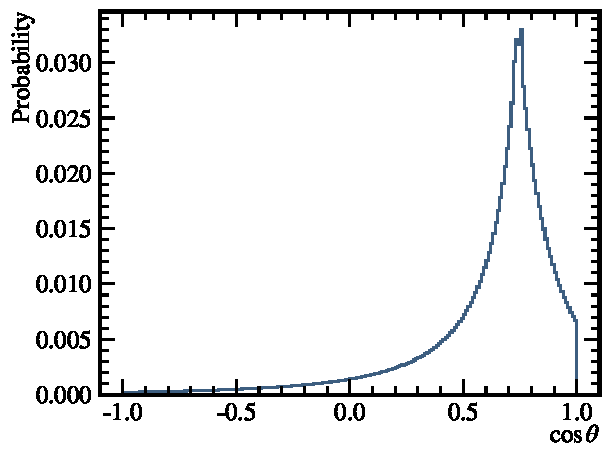
\includegraphics[page=1,width=\textwidth]{reconstruction/emmisionProfile/20.pdf}
		\caption{\SI{20}{MeV} electron}
		\label{fig:theta20mev}
	\end{subfigure}
	\caption{The relationship of emission probability with $\cos\theta$.}
	\label{fig:thetaemmision}
\end{figure}

\begin{figure}[h]
	\centering
	\begin{subfigure}{0.45\textwidth}
		\includegraphics[page=2,width=\textwidth]{reconstruction/emmisionProfile/2.pdf}
		\caption{\SI{2}{MeV} electron}
		\label{fig:s2mev}
	\end{subfigure}
	\hfill
	\begin{subfigure}{0.45\textwidth}
		\includegraphics[page=2,width=\textwidth]{reconstruction/emmisionProfile/5.pdf}
		\caption{\SI{5}{MeV} electron}
		\label{fig:s5mev}
	\end{subfigure}

	\vspace{\baselineskip}

	\begin{subfigure}{0.45\textwidth}
		\includegraphics[page=2,width=\textwidth]{reconstruction/emmisionProfile/10.pdf}
		\caption{\SI{10}{MeV} electron}
		\label{fig:s10mev}
	\end{subfigure}
	\hfill
	\begin{subfigure}{0.45\textwidth}
		\includegraphics[page=2,width=\textwidth]{reconstruction/emmisionProfile/20.pdf}
		\caption{\SI{20}{MeV} electron}
		\label{fig:s20mev}
	\end{subfigure}
	\caption{The relationship of emission probability with $s$.}
	\label{fig:semmision}
\end{figure}


\begin{figure}[h]
	\centering
	\begin{subfigure}{0.45\textwidth}
		\includegraphics[page=3,width=\textwidth]{reconstruction/emmisionProfile/2.pdf}
		\caption{\SI{2}{MeV} electron}
		\label{fig:ts2mev}
	\end{subfigure}
	\hfill
	\begin{subfigure}{0.45\textwidth}
		\includegraphics[page=3,width=\textwidth]{reconstruction/emmisionProfile/5.pdf}
		\caption{\SI{5}{MeV} electron}
		\label{fig:ts5mev}
	\end{subfigure}

	\vspace{\baselineskip}

	\begin{subfigure}{0.45\textwidth}
		\includegraphics[page=3,width=\textwidth]{reconstruction/emmisionProfile/10.pdf}
		\caption{\SI{10}{MeV} electron}
		\label{fig:ts10mev}
	\end{subfigure}
	\hfill
	\begin{subfigure}{0.45\textwidth}
		\includegraphics[page=3,width=\textwidth]{reconstruction/emmisionProfile/20.pdf}
		\caption{\SI{20}{MeV} electron}
		\label{fig:ts20mev}
	\end{subfigure}
	\caption{The relationship of emission probability with $s$ and $\cos\theta$.}
	\label{fig:tsemmision}
\end{figure}

\begin{figure}
	\begin{center}
		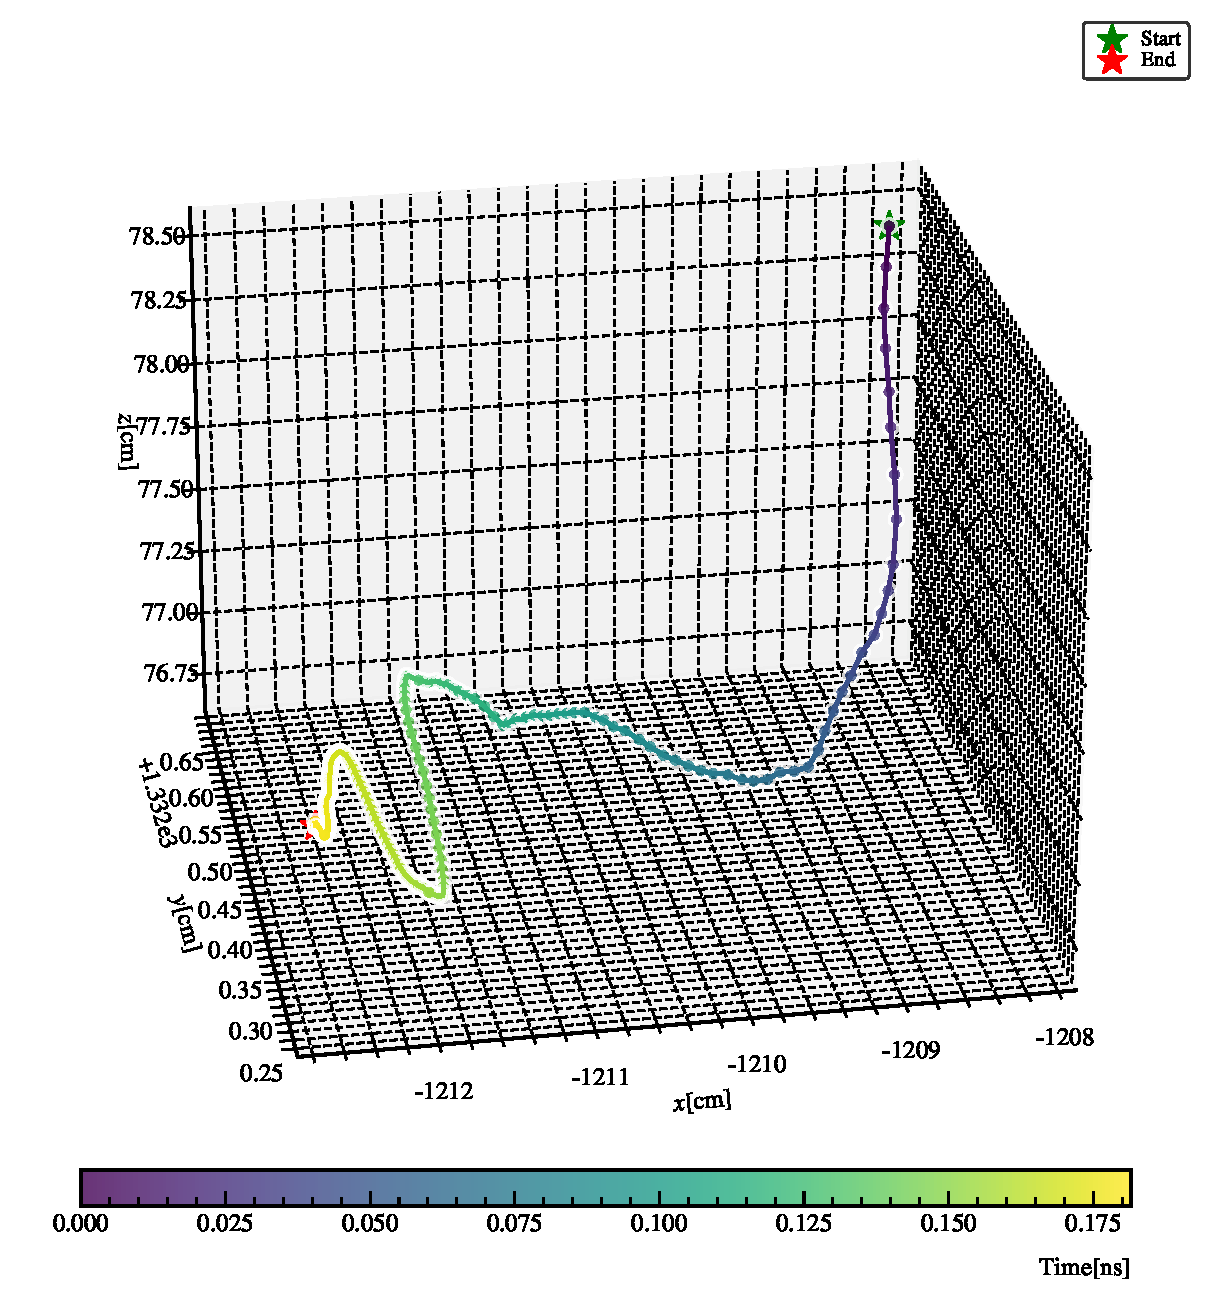
\includegraphics[width=\textwidth]{reconstruction/emmisionProfile/multiscatter.pdf}
	\end{center}
	\caption{An example of a \SI{10}{MeV} electron undergoing multiple scattering.}
	\label{fig:multipleScattering}
\end{figure}

Through Gaussian fitting as shown in Fig~\ref{fig:yield_gauss_fit} in simulation, we obtain the total number of photons emitted at various energies and calculate the Cherenkov photon yield. After linear fitting, we obtain the relationship between light yield and momentum: $\phi(p)=1182\times p-956$.
\begin{figure}[h]
	\centering
	\begin{subfigure}{0.45\textwidth}
		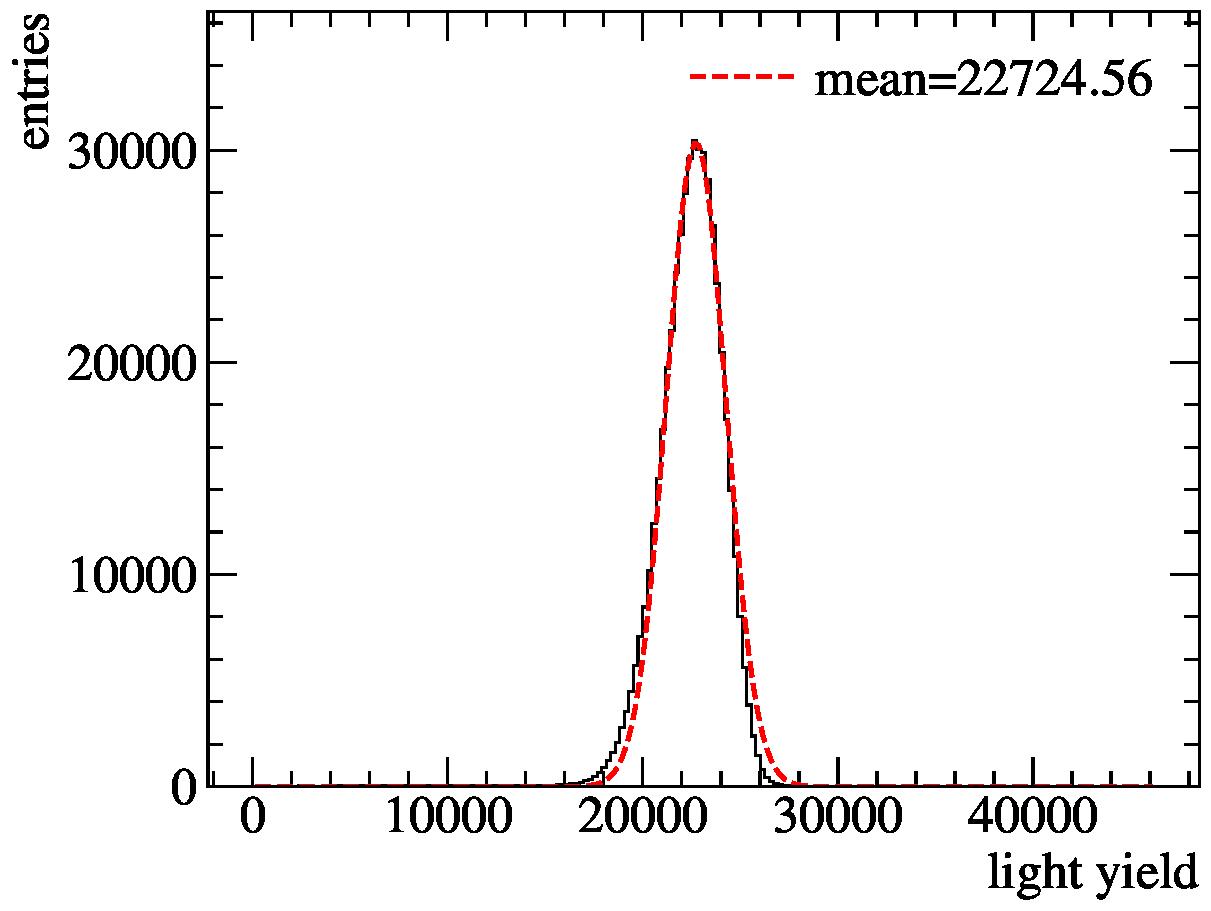
\includegraphics[width=\textwidth]{reconstruction/emmisionProfile/yield_gauss_fit_20.pdf}
		\caption{An example of Gaussian fit for light yield.}
		\label{fig:yield_gauss_fit}
	\end{subfigure}
	\hfill
	\begin{subfigure}{0.45\textwidth}
		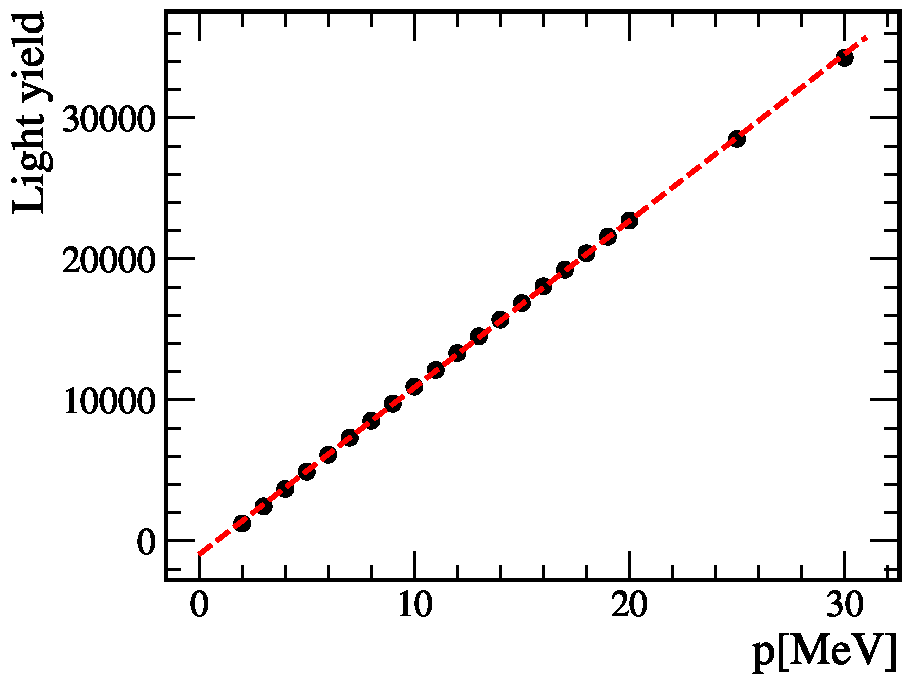
\includegraphics[width=\textwidth]{reconstruction/emmisionProfile/phip.pdf}
		\caption{\SI{5}{MeV} electron}
		\label{fig:yield_fit}
	\end{subfigure}
	\caption{The relationship of emission probability with $s$ and .}
\end{figure}

\subsection{The calculation of direct light}
After establishing the coordinate system, we can readily determine the number of photons received by a specific PMT when an electron is incident.
\begin{equation}
	\mu_{\mathrm{dir}}=\int ds g(p,s,\cos\theta)\phi(p)\Omega(R)T(R)\epsilon(\eta)
	\label{equ:directLight}
\end{equation}
\begin{itemize}
	\item $R$ is the distance between the position of electron and the PMT.
	\item $\Omega(R)$ is the solid angle factor of PMT.
	\item $T(R)$ is the light transmission factor.
	\item $\epsilon(\eta)$ is the PMT angular acceptance of PMT, and $\eta$ is the incident angle of light when captured by PMT.
\end{itemize}

\subsubsection{The solid angle factor}
The main PMTs employed in JUNO are 20-inch with a radius of $a=SI{0.622}{m}$. And we can calculate the solid angle of PMT by Eq.~\eqref{equ:solid}.
\begin{equation}
	\Omega(R)=\frac{\pi a^2}{4\pi(R^2+a^2)}\times (4\pi)=\frac{\pi a^2}{R^2+a^2}
	\label{equ:solid}
\end{equation}
In this approximation, the geometric shape of the PMT is ignored and approximated by a circular wafer. This approximation remains valid only when PMTs are sufficiently distant from the particle. In JUNO, PMTs are mounted at around \SI{19.5}{m} , while our region of interest lies within \SI{17.7}{m}. Based on SK's experience, the approximation holds effectively at radial distances $R > \SI{1.5}{m}$.

\subsubsection{The transmission factor}
In our work, we just use Eq.~\eqref{eq:att}, and the attenuation length $L^{a}$ is \SI{75}{m}.
\begin{equation}
	T(R) = \exp(-R/L^{a})
	\label{eq:att}
\end{equation}

\subsubsection{PMT angular accptance}
$\epsilon(\cos\eta)$ serves as a correction term for the approximation of the PMT wafer, describing the probability of photons being received by the PMT when incident from different directions. We extracted the particles at the same distance from the PMT in the simulation and counted the number of photons received by the PMT, as shown in Fig.~\ref{fig:eta_stat}. We performed a "normalization" calculation of the probability using the number of photons directly incident on the PMT, as shown in Fig.~\ref{fig:cd_norm} and \ref{fig:buffer_norm}. Then we extracted the probability distributions at different $\cos\eta$ values and fitted them with a Gaussian distribution, as shown in Fig.~\ref{fig:eta_gauss_fit}. Thus, we obtained the variation curve of $\epsilon(\cos\eta)$ and fitted it with a polynomial, as illustrated in Fig.~\ref{fig:eta_fit}. Whether it is in CD or buffer, a cut-off point can be observed. This is due to the mutual occlusion between the boundary of the detector and the PMT.

\begin{figure}[h]
	\centering
	\begin{subfigure}{0.45\textwidth}
		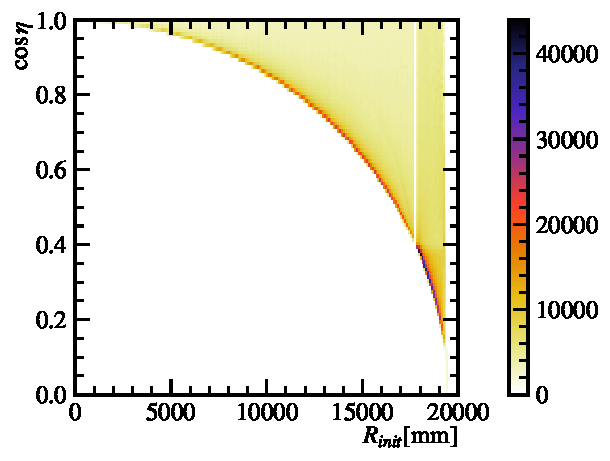
\includegraphics[page=1, width=\textwidth]{reconstruction/eta/fig.pdf}
		\caption{}
		\label{fig:eta_init}
	\end{subfigure}
	\hfill
	\begin{subfigure}{0.45\textwidth}
		\includegraphics[page=2, width=\textwidth]{reconstruction/eta/fig.pdf}
		\caption{}
		\label{fig:eta_R}
	\end{subfigure}
	\caption{\subref{fig:eta_init} is the position distribution, $R_{init}$ is the initial position of \SI{4}{MeV} electron.The boundary of the detector is at \SI{17.7}{m}. There is an acrylic spherical shell with a thickness of \SI{12}{cm}. The area between 17.7 and \SI{19.5}{m} is the buffer.
		\subref{fig:eta_R} shows the relationship between $R$ and $\cos\eta$. The boundary of the two distributions is the acrylic spherical shell.}
	\label{fig:eta_stat}
\end{figure}

\begin{figure}[h]
	\centering
	\begin{subfigure}{0.45\textwidth}
		\includegraphics[page=3, width=\textwidth]{reconstruction/eta/fig.pdf}
		\caption{}
		\label{fig:cd_norm}
	\end{subfigure}
	\hfill
	\begin{subfigure}{0.45\textwidth}
		\includegraphics[page=4, width=\textwidth]{reconstruction/eta/fig.pdf}
		\caption{}
		\label{fig:buffer_norm}
	\end{subfigure}
	\hfill
	\begin{subfigure}{0.45\textwidth}
		\includegraphics[page=45, width=\textwidth]{reconstruction/eta/cd.pdf}
		\caption{}
		\label{fig:eta_gauss_fit}
	\end{subfigure}
	\caption{\subref{fig:cd_norm} and \subref{fig:buffer_norm} are the normalized probability distribution. \subref{fig:eta_gauss_fit} is an example of Gaussian fit.}
	\label{fig:eta_gassian_fit}
\end{figure}

\begin{figure}[h]
	\centering
	\begin{subfigure}{0.45\textwidth}
		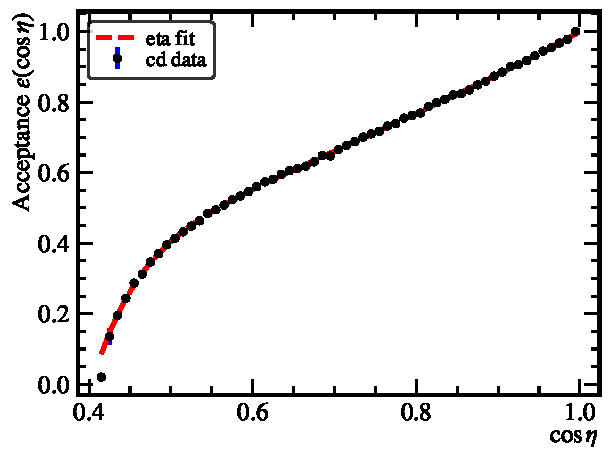
\includegraphics[page=1, width=\textwidth]{reconstruction/eta/fit.pdf}
		\caption{}
		\label{fig:eta_cd}
	\end{subfigure}
	\hfill
	\begin{subfigure}{0.45\textwidth}
		\includegraphics[page=2, width=\textwidth]{reconstruction/eta/fit.pdf}
		\caption{}
		\label{fig:eta_buffer}
	\end{subfigure}
	\caption{The relationship between acceptance~$\epsilon$ and $\cos\eta$ of when event in CD~\subref{fig:eta_cd} and in buffer~\subref{fig:eta_buffer}. }
	\label{fig:eta_fit}
\end{figure}

\subsubsection{The prediction of direct light}
For a single photon, we can combine its propagation process and the process of being captured by the PMT and define it as the photon reception function \(J=\Omega(R)T(R)\epsilon(\eta)\). Given the vertex and direction, this propagation process is only related to the generation position of the photon, that is, the distance from the photon generation point to the vertex. We can write \(J\) as a function of \(s\) and perform a polynomial expansion, retaining the second-order approximation, as Eq.~\eqref{eq:jsApp} and the approximate performance is as shown in Fig.~\ref{fig:js}. Under this approximation, we can select 3 points to calculate the line. In the algorithm implementation, this can be quickly solved through methods such as matrix inversion.
\begin{equation}
	J(s)=\Omega(R)T(R)\epsilon(\eta)\approx j_0 + j_1s+j_2s^2
	\label{eq:jsApp}
\end{equation}

\begin{figure}
	\begin{center}
		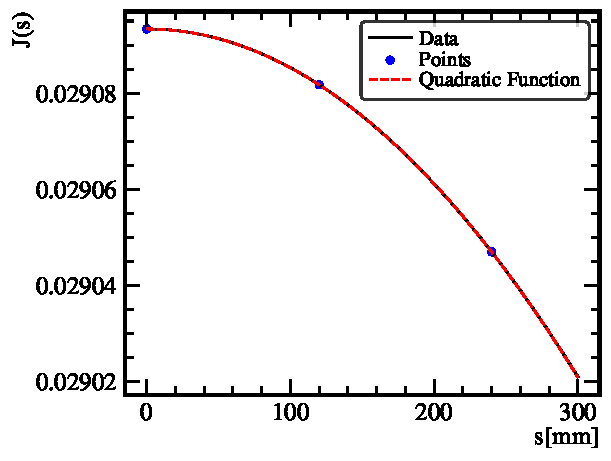
\includegraphics[width=0.5\textwidth]{reconstruction/js.pdf}
	\end{center}
	\caption{An example of second-order approximation to calculate $J(s)$.}
	\label{fig:js}
\end{figure}
Thus far, we can decouple the process of photon generation from the process of photon capture, as shown in Eq.~\eqref{eq:mudir}.
\begin{equation}
	\begin{aligned}
		\mu_{\mathrm{dir}} & =\int ds g(p,s,\cos\theta)\phi(p)\Omega(R)T(R)\epsilon(\eta) \\
		                   & \approx \int ds g(p,s,\cos\theta)\phi(p)(j_0 + j_1s+j_2s^2)  \\
		                   & =\phi(p)(I_0j_0+I_1j_1+I_2j_2)                               \\
	\end{aligned}
	\label{eq:mudir}
\end{equation}
Where $I_i = \int ds g(p,s,\cos\theta)s^i$ is a function of $p, R, \cos\theta$ and represents the emission proportion of Cherenkov photons at a certain relative position. We can complete this integral calculation before the reconstruction.
Due to the relatively large differences in the integration range and emission spectrum at different momenta, we calculate the value of \(I\) for each momentum. Then, we perform a polynomial approximation fitting for momentum and \(I\), as shown in Fig.~\ref{fig:I_fit}. We create a grid with the fitting coefficients in terms of \(R\) and \(\cos\theta\). During the reconstruction process, by looking up different values of \(R\) and \(\cos\theta\) and invoking the corresponding polynomials for calculation, the reconstruction efficiency can be significantly improved.
\begin{figure}[h]
	\centering
	\begin{subfigure}{0.5\textwidth}
		\centering
		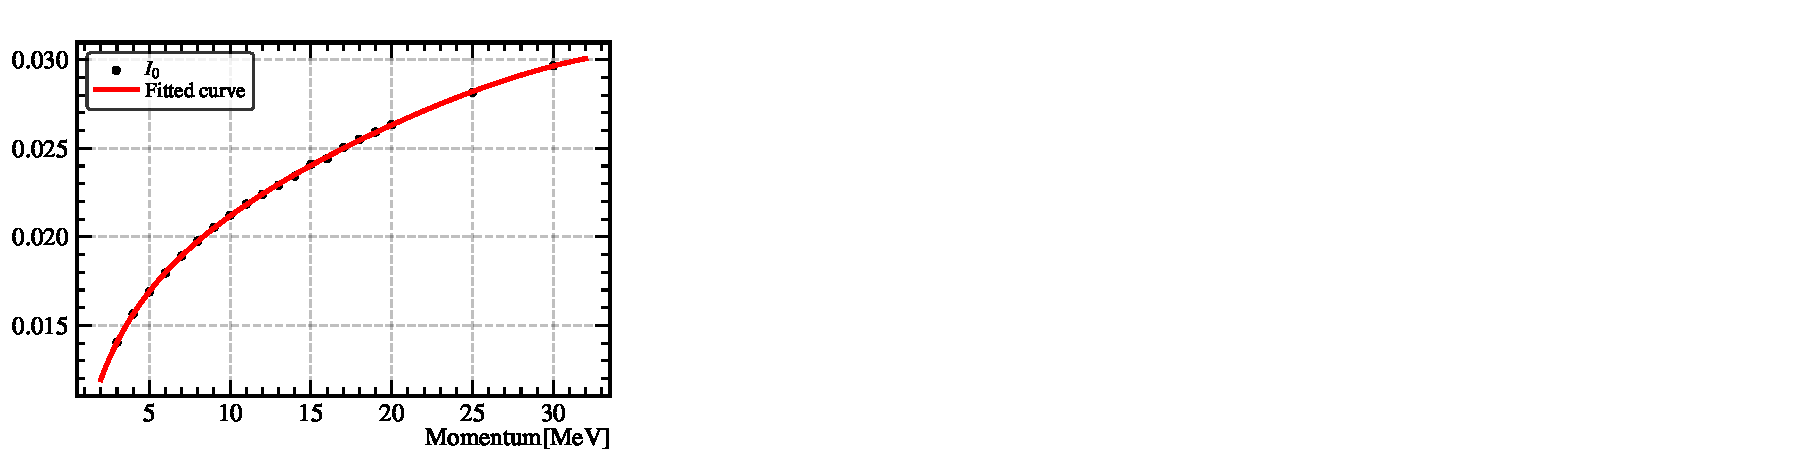
\includegraphics[width=0.8\textwidth]{reconstruction/I0.pdf}
		\caption{$I_0$}
		\label{fig:I0}
	\end{subfigure}% 
	\hfill
	\begin{subfigure}{0.5\textwidth}
		\centering
		
\includegraphics[width=0.8\textwidth]{reconstruction/I1.pdf}
		\caption{$I_1$}
		\label{fig:I1}
	\end{subfigure}%
	\hfill
	\begin{subfigure}{0.5\textwidth}
		\centering
		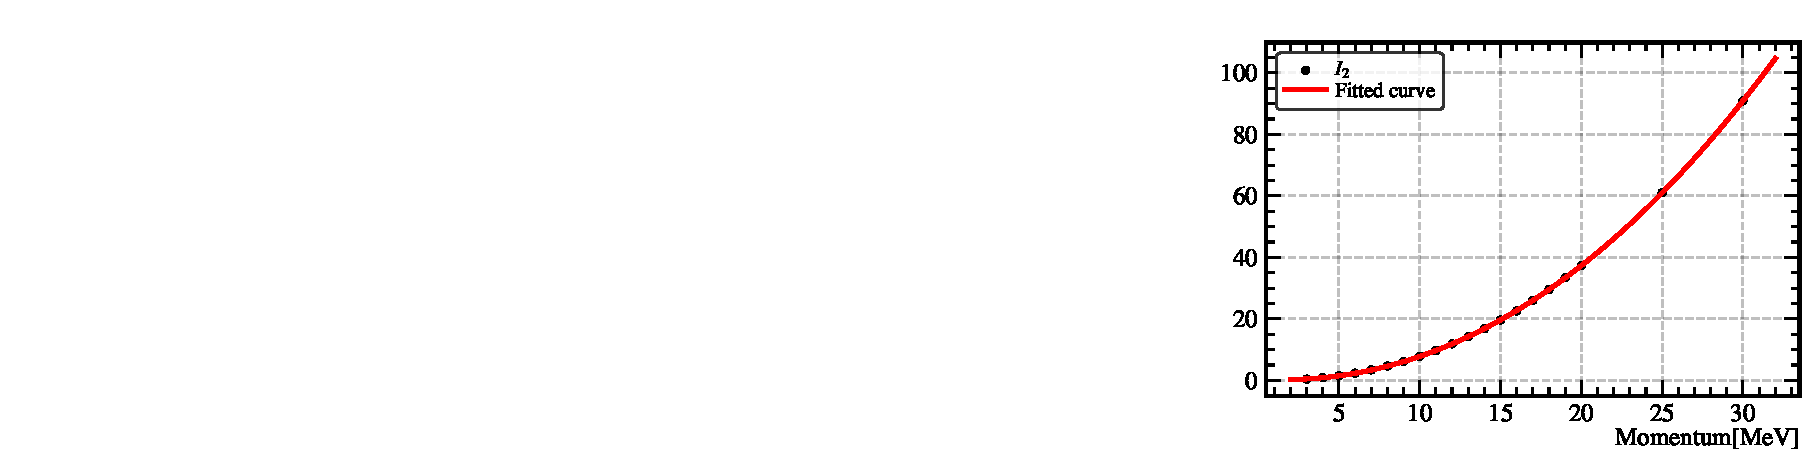
\includegraphics[width=0.8\textwidth]{reconstruction/I2.pdf}
		\caption{$I_2$}
		\label{fig:I2}
	\end{subfigure}
	\caption{The fit of $I_i,i=0,1,2$ when $R=\SI{15}{m},\cos\theta=0.72$}
	\label{fig:I_fit}
\end{figure}

\subsection{The prediction of indirect light based on direct light}
During the propagation of Cherenkov light, scattering and refraction inevitably occur. Perhaps after a long propagation process, these photons finally reach PMTs and are captured. This makes it necessary to take into account the indirect photons when considering the expected number of photons. For a given vertex and momentum, we can perform an integration along the particle track for indirect light, just as we do for direct light. Since indirect light evolves from directly incident light, we can use a proportionality ratio $A(s)$ to characterize the indirect light component.
\begin{equation}
	\begin{aligned}
		\mu_{\mathrm{ind}} & =\int ds g(p,s,\cos\theta)\phi(p)\Omega(R)T(R)\epsilon(\eta)A(s) \\
		                   & \approx \int ds g(p,s,\cos\theta)\phi(p)(j_0 + j_1s+j_2s^2)A(s)  \\
	\end{aligned}
	\label{eq:indir}
\end{equation}
Through ray tracing in the simulation, we are able to differentiate between direct light and indirect light. We perform binning statistics using \(R\) and \(\cos\theta\), as shown in the Fig.~\ref{fig:fig:dir} and \ref{fig:ind}. At the same time, it is sufficient to depict the corresponding relationship between \(A\) and the relative positions \(R\) and \(\cos\theta\) to make a scatter table, as illustrated in Fig.~\ref{fig:ratio}. Near the vertex and around the Cherenkov angle, the ratio of indirect light to direct light is about 0.1. When far from the vertex and the Cherenkov angle, indirect light is dominant. For low-energy electrons, the track length of their motion typically ranges from several centimeters to over ten centimeters. In the scattering table employed, the bin width of \(R\) is set to \(10\) cm. Under such circumstances, the approximation \(A(s)=A(s = 0)\) is highly adequate. Consequently, the integral of the indirect light can be expressed as Eq.~\eqref{eq:indir_s}.
\begin{equation}
	\begin{aligned}
		\mu_{\mathrm{ind}} & \approx \int ds g(p,s,\cos\theta)\phi(p)(j_0 + j_1s+j_2s^2)A(s) \\
		                   & \approx \phi(p)(I_0j_0+I_1j_1+I_2j_2)A(s=0)                     \\
	\end{aligned}
	\label{eq:indir_s}
\end{equation}
The final light prediction can be $\mu_p=\mu_{dir}+\mu_{ind}=\phi(p)(I_0j_0+I_1j_1+I_2j_2)(1+A(s=0))$. After considering the PDE of PMT, the prediction of PE should be $\mu=\varepsilon\mu_p=\varepsilon\phi(p)(I_0j_0+I_1j_1+I_2j_2)(1+A(s=0))$
\begin{figure}[h]
	\centering
	\begin{subfigure}{0.5\textwidth}
		\centering
		\includegraphics[page=1,width=0.8\textwidth]{reconstruction/scatter_ratio.pdf}
		\caption{direct light}
		\label{fig:dir}
	\end{subfigure}% 
	\hfill
	\begin{subfigure}{0.5\textwidth}
		\centering
		\includegraphics[page=2,width=0.8\textwidth]{reconstruction/scatter_ratio.pdf}
		\caption{indirect light}
		\label{fig:ind}
	\end{subfigure}%
	\hfill
	\begin{subfigure}{0.5\textwidth}
		\centering
		\includegraphics[page=5,width=0.8\textwidth]{reconstruction/scatter_ratio.pdf}
		\caption{ratio of indirect and direct light}
		\label{fig:ratio}
	\end{subfigure}
	\caption{The scatter table}
	\label{fig:scatterTable}
\end{figure}

\subsection{The timing response}
In Cherenkov reconstruction, photons are emitted along the Cherenkov angle rather than isotropically. Consequently, when only charge information is utilized for reconstruction, accurately determining the position becomes challenging. Time serves to characterize both the emission properties and the distance characteristics during propagation. To a certain degree, it offsets the limitations of relying solely on charge information. Thus, in the detector response, time is an essential parameter. As depicted in Fig.~\ref{fig:tres_define}, in the reconstruction process, we employ the residual time obtained by subtracting the time of flight, as defined in Eq.~\eqref{eq:trea_def}.
\begin{equation}
	t_{\mathrm{res},i} = t_i - t - s_{\mathrm{mid}}/c - \frac{|\boldsymbol{P}_{\mathrm{PMT}}^i - \boldsymbol{x} - s_{\mathrm{mid}}\widehat{\overrightarrow{d} } |}{c_w}
	\label{eq:trea_def}
\end{equation}
Where $t$ is the event time, $\boldsymbol{x}$ is the vertex, $t_i$ is the hit time at $i$-th PMT and $\boldsymbol{P}_{\mathrm{PMT}}^i$ is the position of $i$-th PMT.
\begin{figure}
	\begin{center}
		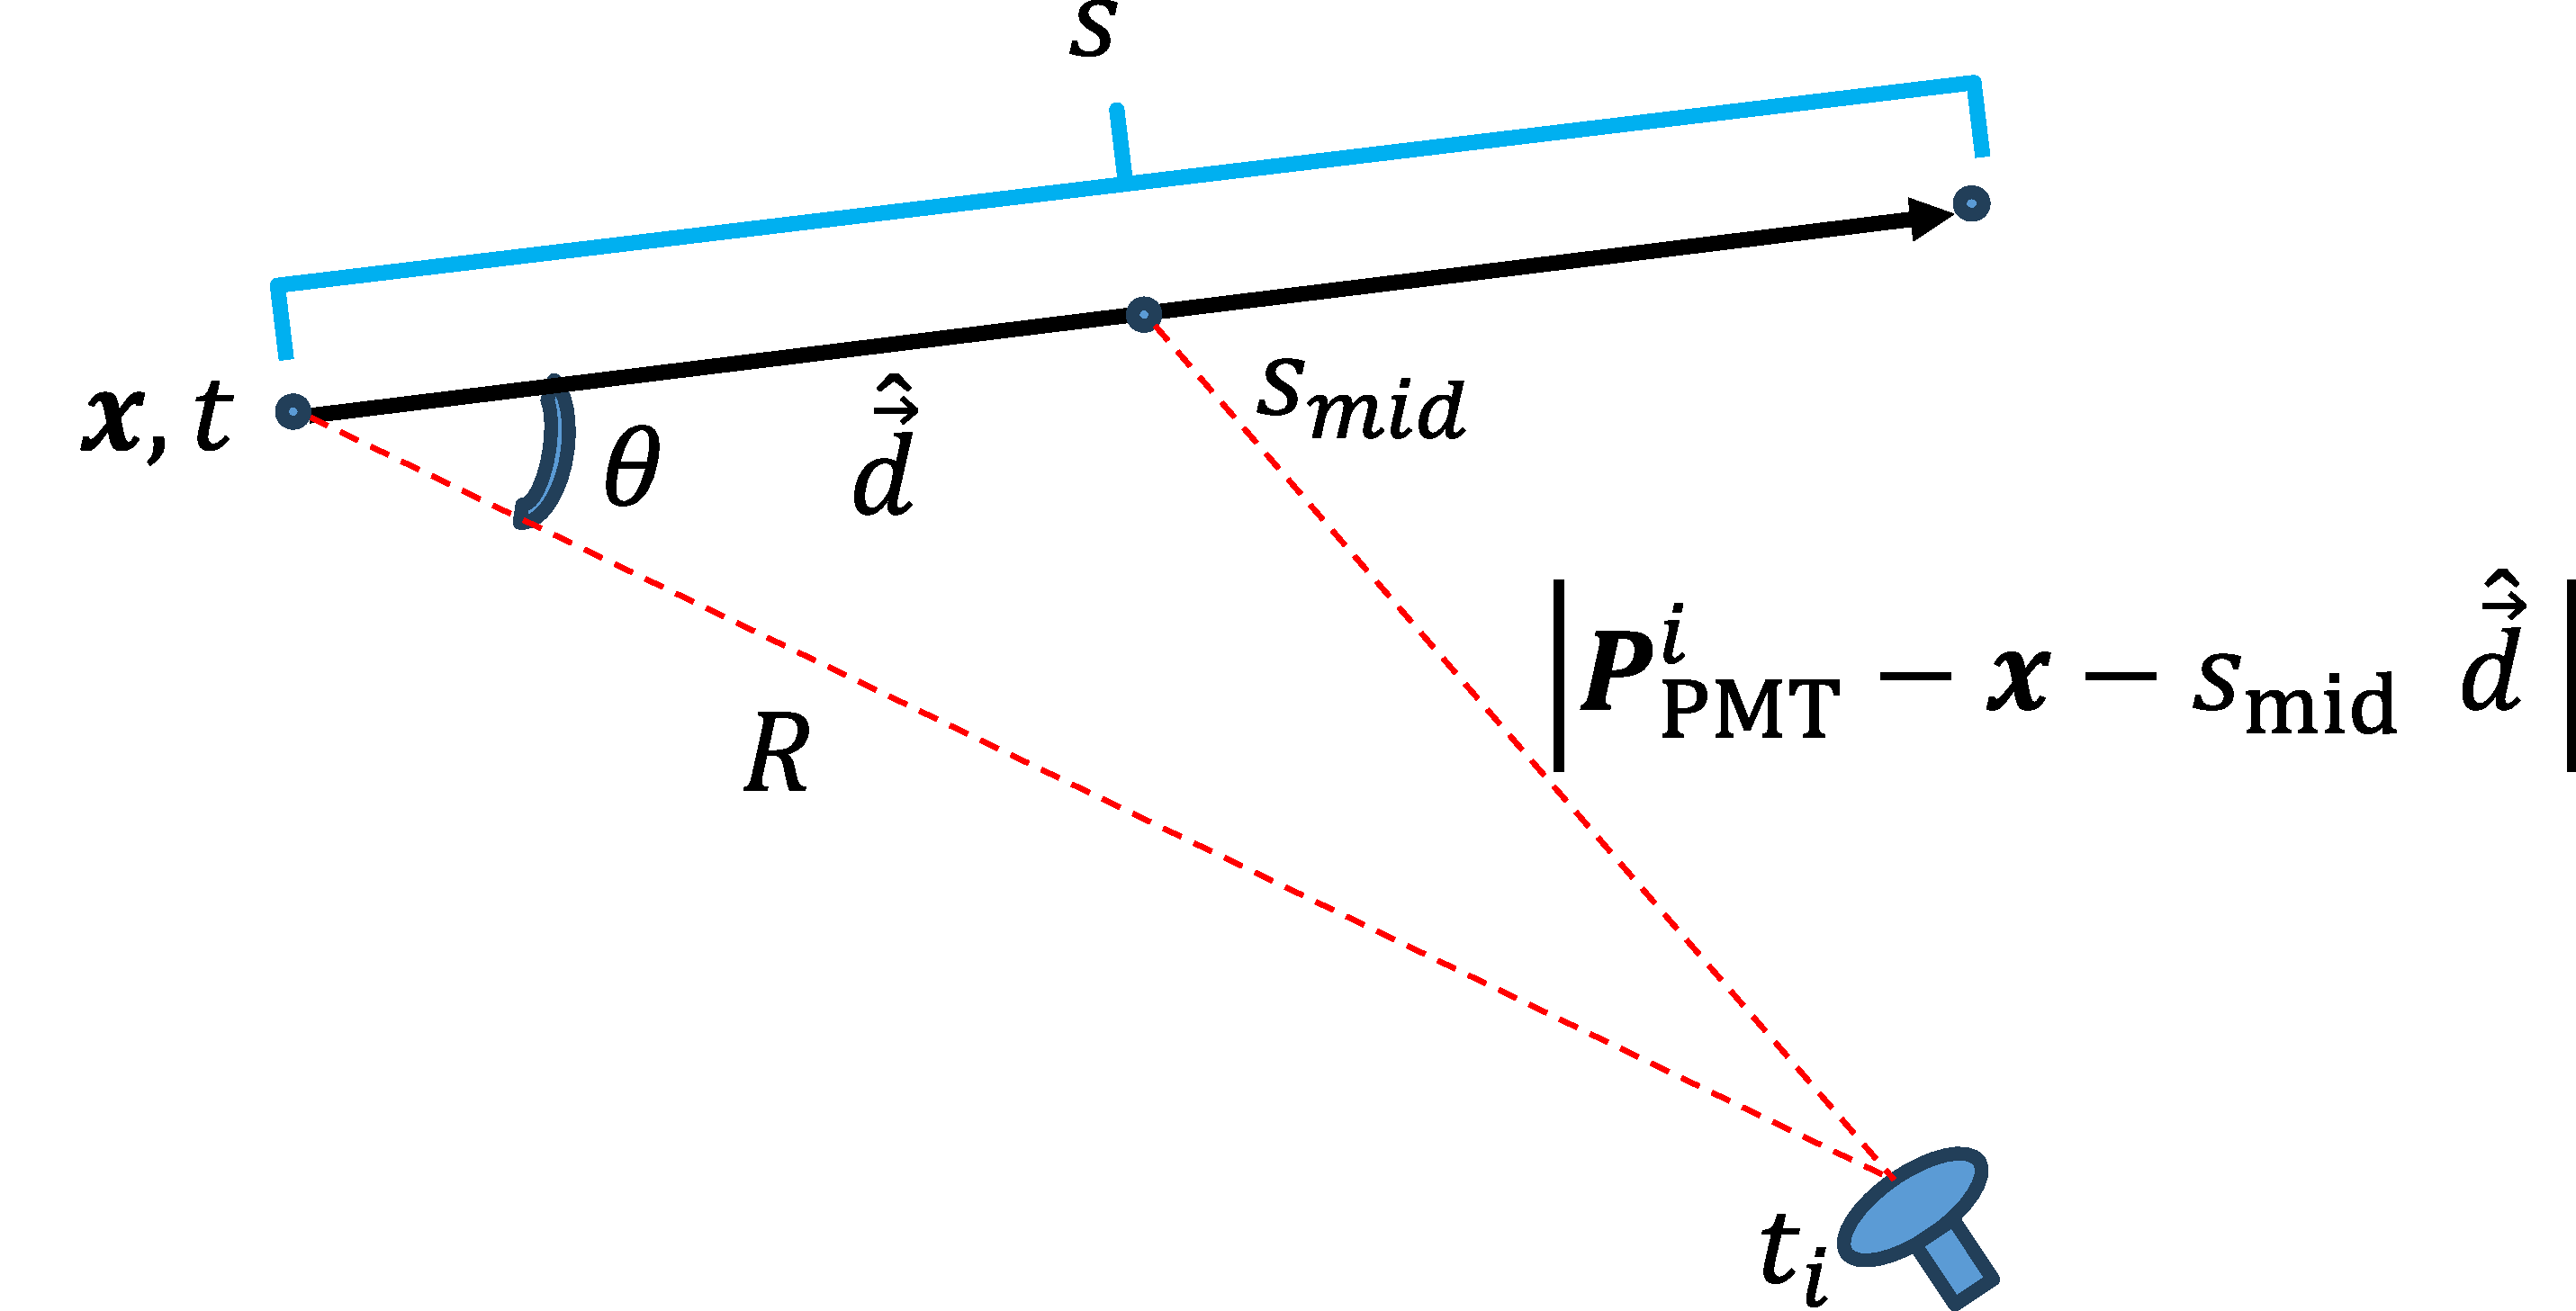
\includegraphics[width=0.8\textwidth]{reconstruction/timepdf/time.pdf}
	\end{center}
	\caption{The definition of residual time.}
	\label{fig:tres_define}
\end{figure}
In fiTQun, following the classification of the residual time of the direct light according to the expected number, the mean and standard deviation of the residual time distribution are derived through Gaussian fitting. Subsequently, the means and variances under different expectations are fitted to accomplish the parameterization of the time response. However, this approach is not conducive to considering factors such as TTS. In this study, we directly classify the residual time using the relative distance, approximate the probability density function~($R_p(t)$) with a histogram, and carry out integration to obtain the corresponding cumulative distribution function~($R_c(t)$), as shown in Fig.~\ref{fig:smear0}. Analogously, by leveraging the histogram, we accomplished the time smearing of the TTS response through convolution, as depicted in Fig.~\ref{fig:smear5}. Given that the maximum TTS of the PMT can attain up to \SI{15}{ns}, we carried out the time convolution smearing for the TTS within the range of 0--\SI{15}{ns}.

\begin{figure}[h]
	\centering
	\begin{subfigure}{0.5\textwidth}
		\centering
		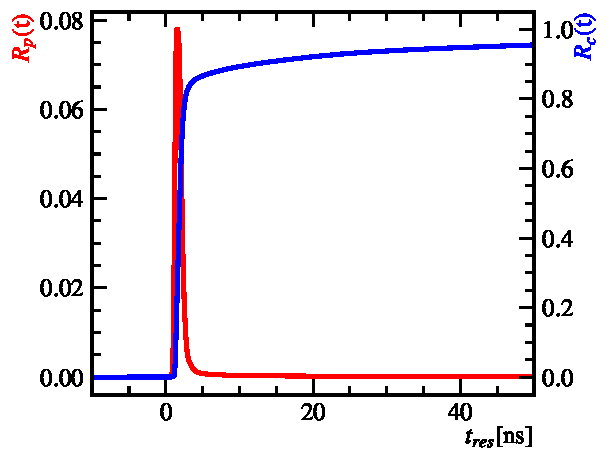
\includegraphics[page=1, width=0.9\textwidth]{reconstruction/timepdf/sub_0.pdf}
		\caption{Without TTS smearing}
		\label{fig:smear0}
	\end{subfigure}% 
	\begin{subfigure}{0.5\textwidth}
		\centering
		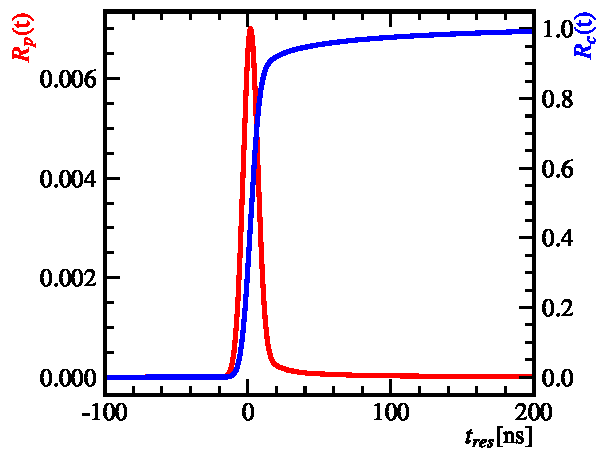
\includegraphics[page=1, width=0.9\textwidth]{reconstruction/timepdf/sub_5.pdf}
		\caption{With \SI{5}{ns} TTS smearing.}
		\label{fig:smear5}
	\end{subfigure}
	\caption{The PDF and CDF of $t_{\mathrm{res}}$.}
	\label{fig:time}
\end{figure}

\subsection{The DCR in reconstruction}
From PMT calibration in Sec.~\ref{sec:dcr}, the DCR is determined to be exceedingly high. In the course of the reconstruction process, considering that the dark noise adheres to a homogeneous Poisson intensity process within the time window, the probability of occurrence within a unit time window can be approximated by DCR. Given an intensity of $b$, the predicted PE should be $\mu+b(\overline{t}-\underline{t})$, and the time PDF should be $f_t(t_i)=\mu R_p(t_{\mathrm{res},i})+b$. And our likelihood is as shown in Eq.~\eqref{eq:likelihood_dcr}.
\begin{equation}
	\begin{aligned}
		\mathcal{L}
		 & = \prod_{j \in \{N_j>0\}} \frac{1}{(N_j-1)!}
		\exp\Big[ -\mu_j\big(R_c(\overline{t}_{\mathrm{res},j}) - R_c(\underline{t}_{\mathrm{res},j})\big) - b(\overline{t}_{\mathrm{res},j}-\underline{t}_{\mathrm{res},j})\Big]                                          \\
		 & \quad \times \big( \mu R_p(t_{\mathrm{res},j})+b \big)
		\quad \times \Big( \mu \big( R_c(\overline{t}_{\mathrm{res},j}) - R_c(\underline{t}_{\mathrm{res},j}) \big) + b(\overline{t}_{\mathrm{res},j} - t_{\mathrm{res},j}) \Big)^{N_j-1}                                  \\
		 & \quad \times \prod_{j \in \{N_j=0\}} \exp\Big[ -\mu\big(R_c(\overline{t}_{\mathrm{res},j}) - R_T(\underline{t}_{\mathrm{res},j})\big) - b(\overline{t}_{\mathrm{res},j} - \underline{t}_{\mathrm{res},j}) \Big]
	\end{aligned}
	\label{eq:likelihood_dcr}
\end{equation}

\subsection{Use MCMC for extremization}
To avoid the influence of local extrema, we use Markov Chain Monte Carlo~(MCMC) for extremization~\cite{MCMC}.
To expedite convergence, we employ the simulated annealing method~\cite{prefit}. Specifically, we anneal the TTS from \SI{50}{ns} to the actual calibrated result in Sec.~\ref{sec:tts}.
In each event, we sample a total of 3,000 steps. We use the results of the last 300 steps and calculate the average as the reconstruction result.

\subsection{The preliminary reconstruction}
Prior to the likelihood-based reconstruction, a faster preliminary reconstruction based on timing information and gridded vertex map is performed to reject unphysical events to  reduce the data volume. In the preliminary reconstruction, two parameters are defined:
\begin{itemize}
	\item score: Dark noise event filter based on residual time distribution and charge-weighted vectors from CD center to PMTs. The closer score is to 0, the more likely the event is a dark noise event
	\item isglass: Glass radioactive event filter developed from the decision tree. Its range is from 0 to 1, and the closer the result is to 1, the more likely the event is a glass radioactive event.
\end{itemize}

\section{The parameters definition}
\subsection{The energy related parameters}
For a more accurate description, we define several parameters as shown in Fig.~\ref{fig:dual}.
\begin{itemize}
	\item $n_{10}$: The maximum count of residual time $t_{\mathrm{res}}$ within a
	      \SI{10}{\nano s} bin width
	\item $n_{b}$: The average count of $t_{\mathrm{res}}$ in [-20, -10] and
		      [30,40]\si{\nano s}.
	\item $n_{20}$: The total count of $t_{\mathrm{res}}$ in [-20, 20]\si{\nano s},
	      it is the primary estimation of energy.
	\item $n_c$: The count of $\cos\theta$ in [0.65, 0.85], and the definition of $\theta$ is shown in Fig.~\ref{Fig:Coordinate}.
\end{itemize}

\begin{figure}[h]
	\centering
	\begin{subfigure}{0.5\textwidth}
		\centering
		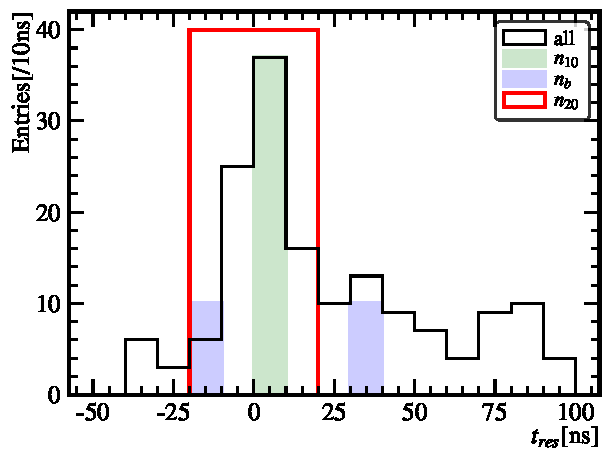
\includegraphics[width=0.9\textwidth]{reconstruction/parameters_Define/tresCount.pdf}
		\caption{The distribution of $t_{\mathrm{res}}$.}
		\label{fig:n20def}
	\end{subfigure}% 
	\begin{subfigure}{0.5\textwidth}
		\centering
		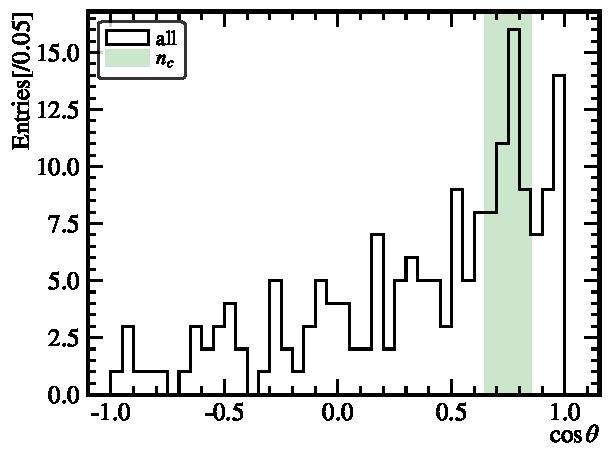
\includegraphics[width=0.9\textwidth]{reconstruction/parameters_Define/cosCount.pdf}
		\caption{The distribution of $\cos\theta$.}
		\label{fig:nc}
	\end{subfigure}
	\caption{The definition of parameters related to energy.}
	\label{fig:dual}
\end{figure}

\subsection{The parameters for reconstruction quality}
There exist two types of background, which can exert a significant impact on our analysis. These include the trigger stemming from pure dark noise and the events originating from PMT radioactivity. To eliminate these backgrounds, we introduce several parameters. To comprehensively assess the performance of each parameter, we simulate the uniform distribution of \SI{2.2}{MeV} Gamma, radioactive events from PMTs, and dark noise trigger events within the detector. Subsequently, reconstruction is performed following the MM trigger.

\subsubsection{Kurtosis test~($k$)}
The value obtained from the Kurtosis test on the residual time distribution is employed to assess the quality of the signal. In the case where the trigger originates from dark noise, the value should be -1.

\subsubsection{Akaike Information Criterion}
Akaike Information Criterion~(AIC) is frequently employed in model selection~\cite{AIC}. In the context of reconstruction, it is utilized to determine whether the trigger originates from noise or a physical event. This Criterion is defined as Eq.~\eqref{eq:aic}
\begin{equation}
	\begin{aligned}
		 & \text{AIC}_v = -2 \ln \mathcal{L}_v + 2k_p \\
		 & \text{AIC}_0 = -2 \ln \mathcal{L}_0
	\end{aligned}
	\label{eq:aic}
\end{equation}
Where $\mathcal{L}$ represents the likelihood of the event with a single vertex, and $k_p$ denotes the number of reconstructed parameters. During the reconstruction process, we also calculate the likelihood of non-vertex events~($\mathcal{L}_0$). In this scenario, we can obtain the AIC criterion:
\begin{equation}
	\delta A = AIC_v - AIC_0 = 14 - 2\ln \mathcal{L}_v + \ln \mathcal{L}_0
	\label{eq:daic}
\end{equation}
By comparing $\delta A$ of dark noise events and \SI{2.2}{MeV} Gamma events, it can be seen that most dark noise events are eliminated, while less than \SI{10}{\%} of Gamma events are removed.
\begin{figure}
	\centering
	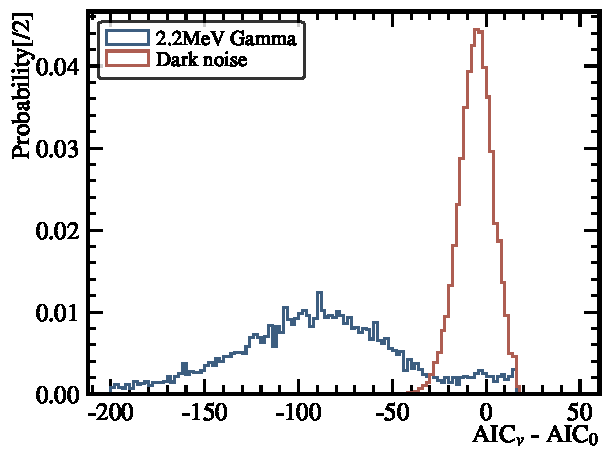
\includegraphics[width=0.45\textwidth]{reconstruction/parameters_Define/AIC_per.pdf}
	\caption{There is obvious difference between dark noise and
		\SI{2.2}{MeV} Gamma. We can optimize it to remove dark noise events.}
\end{figure}

\subsubsection{The likelihood-energy combined Criterion}
We define the likelihood-energy combined criterion as $LE$, as shown in Eq.~\eqref{eq:le}
\begin{equation}
	LE = -\ln \mathcal{L}/n_{20}
	\label{eq:le}
\end{equation}
This criterion is employed to eliminate events stemming from PMT radioactivity. When the cut $LE < 40$ is applied, over \SI{99.99}{\%} of the events from PMT radioactivity are removed, along with approximately \SI{30}{\%} of the \SI{2.2}{MeV} Gamma.
\begin{figure}[h]
	\centering
	\begin{subfigure}{0.5\textwidth} % 宽度调整为0.32(留出间隙)
		\centering
		\includegraphics[page=3, width=0.8\textwidth]{reconstruction/parameters_Define/glass.pdf}
		\caption{\SI{2.2}{MeV} Gamma}
		\label{fig:glass3}
	\end{subfigure}%
	\hfill
	\begin{subfigure}{0.5\textwidth}
		\centering
		\includegraphics[page=6, width=0.8\textwidth]{reconstruction/parameters_Define/glass.pdf}
		\caption{PMT radioactivity}
		\label{fig:glass6}
	\end{subfigure}%
	\hfill
	\begin{subfigure}{0.5\textwidth}
		\centering
		\includegraphics[page=9, width=0.8\textwidth]{reconstruction/parameters_Define/glass.pdf}
		\caption{dark noise events}
		\label{fig:glass9}
	\end{subfigure}
	\caption{The relationship between $\mathcal{L}$ and $n_{20}$.}
	\label{fig:glass_all}
\end{figure}

\subsubsection{The goodness of reconstruction}
When contemplating reconstruction, it is essential to assess the quality of both position and direction. In the case of a successfully reconstructed position, the residual time should be distributed as closely as feasible around zero. For precise direction reconstruction, PMTs adjacent to the Cherenkov ring ought to demonstrate uniform photon acceptance. In accordance with these criteria, we formulate the following two goodness metrics, presented as Eq.~\eqref{eq:goodness}. Finally, we combine these two metrics to obtain the overall goodness of reconstruction, denoted as $G_{vd}=g_v^2-g_d^2$.
\begin{equation}
	\begin{aligned}
		g_v & = \frac{\sum e^{-0.5(t_{\mathrm{res}}/w)^2} e^{-0.5(t_{\mathrm{res}}/\sigma)^2}}{\sum e^{-0.5(t_{\mathrm{res}}/w)^2}}     \\
		g_d & = \frac{1}{2\pi} \left[ \max\left( \phi_i - \frac{2i\pi}{N} \right) - \min\left( \phi_i - \frac{2i\pi}{N} \right) \right] \\
	\end{aligned}
	\label{eq:goodness}
\end{equation}
\begin{itemize}
	\item $w$ and $\sigma$: in this work, $w=\SI{20}{ns}$ and $\sigma$ is the TTS of PMT.
	\item $g_v$: The goodness of position reconstruction.
	\item $g_d$: The goodness of direction, describes the uniformity of the azimuthal angle distribution, as shown in Fig.~\ref{fig:goodness}.
\end{itemize}
\begin{figure}
	\centering
	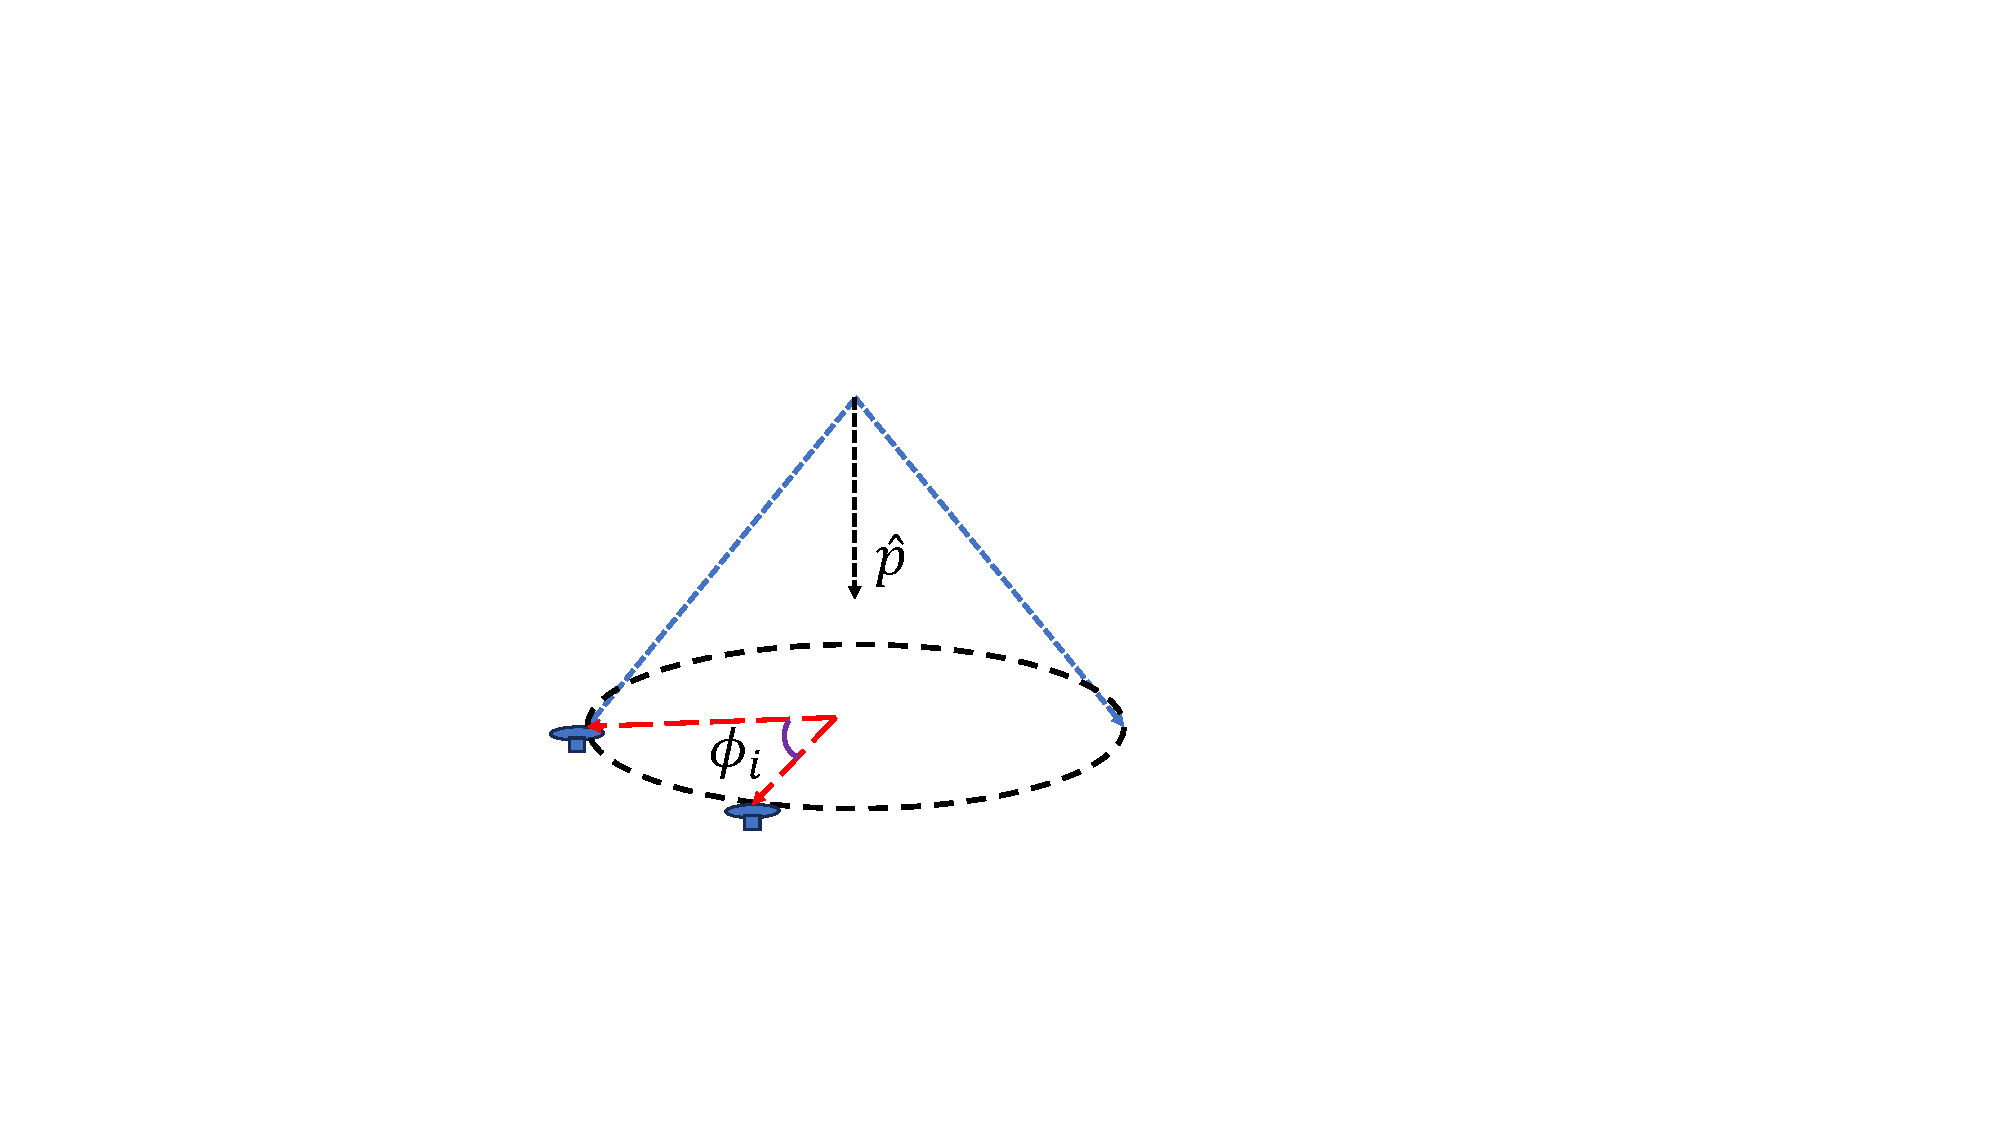
\includegraphics[width=0.45\textwidth]{reconstruction/parameters_Define/gd.pdf}
	\caption{The definition of azimuthal angle in the goodness of direction calculation.}
	\label{fig:goodness}
\end{figure}
\section{The performance of reconstruction in simulation}

To assess the performance of reconstruction, we simulated electrons and \SI{2.2}{MeV} gamma rays and computed the resolution. The information regarding the simulated electrons and Gamma is shown in Table~\ref{tab:particles}. The simulation is conducted based on JUNO software, version J25.1.5. In order to be as close to the actual situation as possible, we update the DCR obtained from the calibration in Sec.~\ref{sec:dcr} into the simulation.
\begin{table}[ht]
	\centering
	\caption{Particles used in simulation}
	\label{tab:particles}
	\begin{tabular}{ccc}
		\toprule
		Particle & Energy~(MeV)                 & Distribution    \\
		\midrule
		$e^-$    & 2, 3, 4, 5, 6, 8, 10, 15, 20 & Uniformly in CD \\
		Gamma    & 2.2                          & Uniformly in CD \\
		\bottomrule
	\end{tabular}
\end{table}

We define the \SI{68.3}{\%} quantile of the distribution of $R_{diff}$ as position resolution, and
the \SI{68.3}{\%} quantile of the distribution of $\theta_{diff}$ as angle resolution, as shown in Fig.~\ref{fig:dir_cal}. For \SI{2.2}{MeV} Gamma, the position resolution is \SI{1.97}{m} and direction resolution is \SI{43.82}{\degree}. It indicates that during the JUNO water phase, we can reconstruct Gamma rays of \SI{2.2}{MeV}. That is to say, we can still reconstruct the n-H capture signal well even though the DCR is pretty high.
\begin{figure}[h]
	\centering
	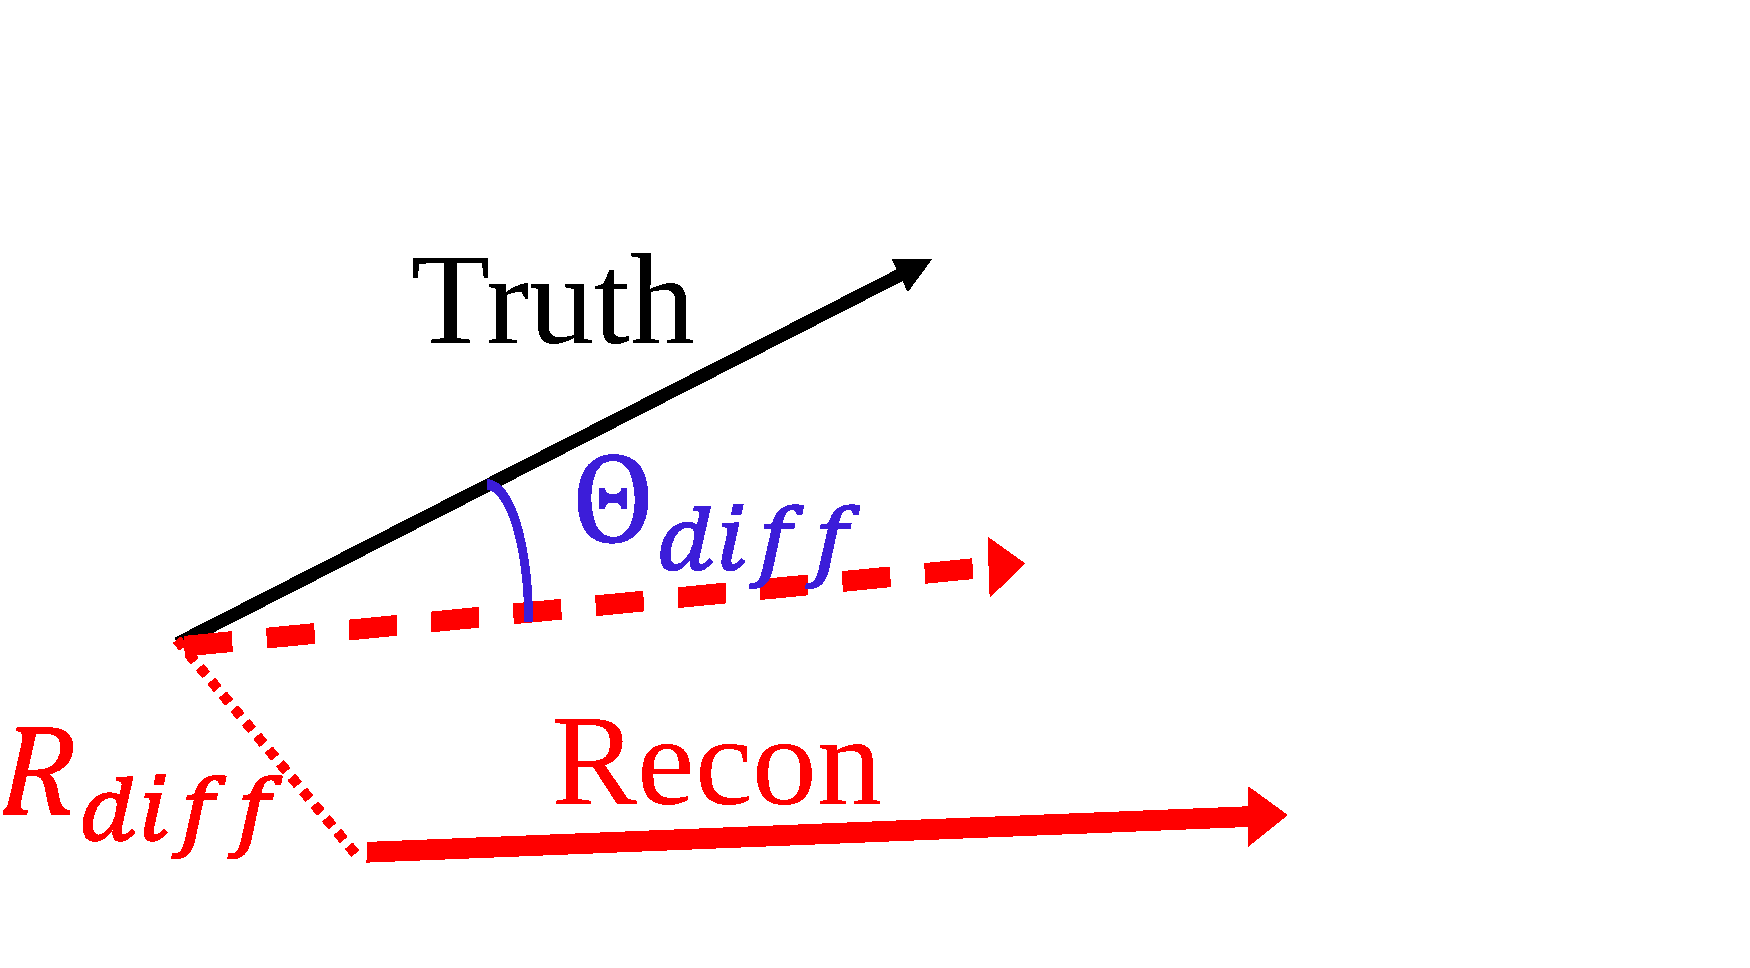
\includegraphics[width=0.3\textwidth]{reconstruction/evalvation.pdf}
	\caption{$R_{diff}$ is the distance between reconstructed position and true position, $\theta_{diff}$ is the angle between reconstructed direction and true direction.}
	\label{fig:evalvation}
\end{figure}

\begin{figure}[h]
	\centering
	\begin{subfigure}{0.5\textwidth} % 宽度调整为0.32(留出间隙)
		\centering
		\includegraphics[page=21,width=0.8\textwidth]{reconstruction/e_res.pdf}
		\caption{Position resolution}
		\label{fig:gamma_pos}
	\end{subfigure}%
	\hfill
	\begin{subfigure}{0.5\textwidth}
		\centering
		\includegraphics[page=22,width=0.8\textwidth]{reconstruction/e_res.pdf}
		\caption{Direction resolution}
		\label{fig:gamma_dir}
	\end{subfigure}%
	\caption{The resolution definition based on \SI{2.2}{MeV} Gamma.}
	\label{fig:dir_cal}
\end{figure}

After calculation the resolution of different electrons, we get the relationship between resolution and electron kinetic energy, as exhibited in Fig.~\ref{fig:res_pos} and Fig.~\ref{fig:dir_pos}. When compared to the position resolution of SK-IV, the position resolution in the water phase of JUNO is relatively lower. This can be attributed to the fact that the PMTs in JUNO exhibit a higher DCR and poorer TTS. At the low-energy regime, a comprehensive modeling of the charge response of Cherenkov has been conducted, resulting in improved directional resolution than SK-III~(SK-IV's direction resolution is the same as SK-III).
\begin{figure}[h]
	\begin{subfigure}{0.5\textwidth}
		\centering
		{\includegraphics[page=19,width=0.8\textwidth]{reconstruction/e_res.pdf}}
		\caption{Position resolution}
		\label{fig:res_pos}
	\end{subfigure}%
	\hfill
	\begin{subfigure}{0.5\textwidth}
		\centering
		{\includegraphics[page=20,width=0.8\textwidth]{reconstruction/e_res.pdf}}
		\caption{Direction resolution}
		\label{fig:dir_pos}
	\end{subfigure}%
	\hfill
	\begin{subfigure}{0.5\textwidth}
		\centering
		{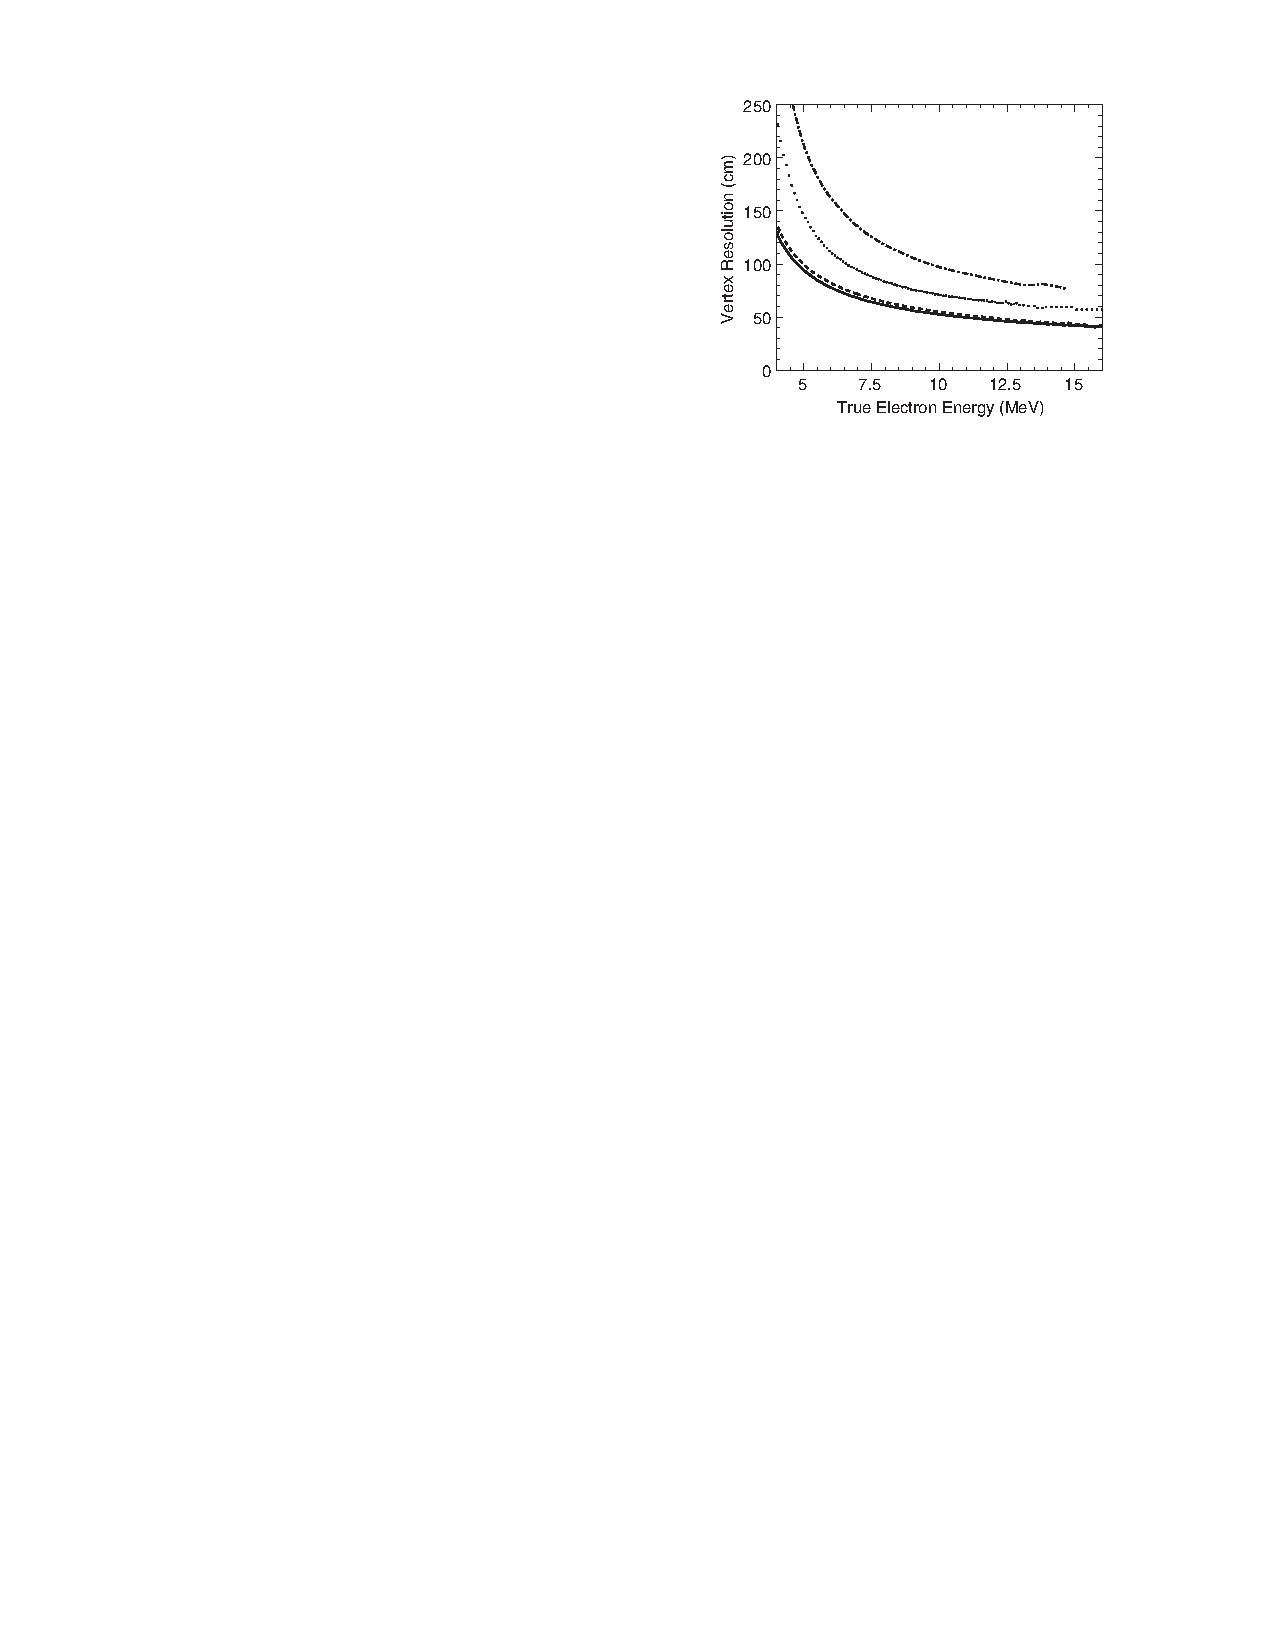
\includegraphics[width=0.8\textwidth]{reconstruction/SK-pos.pdf}}
		\caption{SK's position resolution from SK-IV~\cite{SK4}}
		\label{fig:SKres_pos}
	\end{subfigure}%
	\hfill
	\begin{subfigure}{0.5\textwidth}
		\centering
		{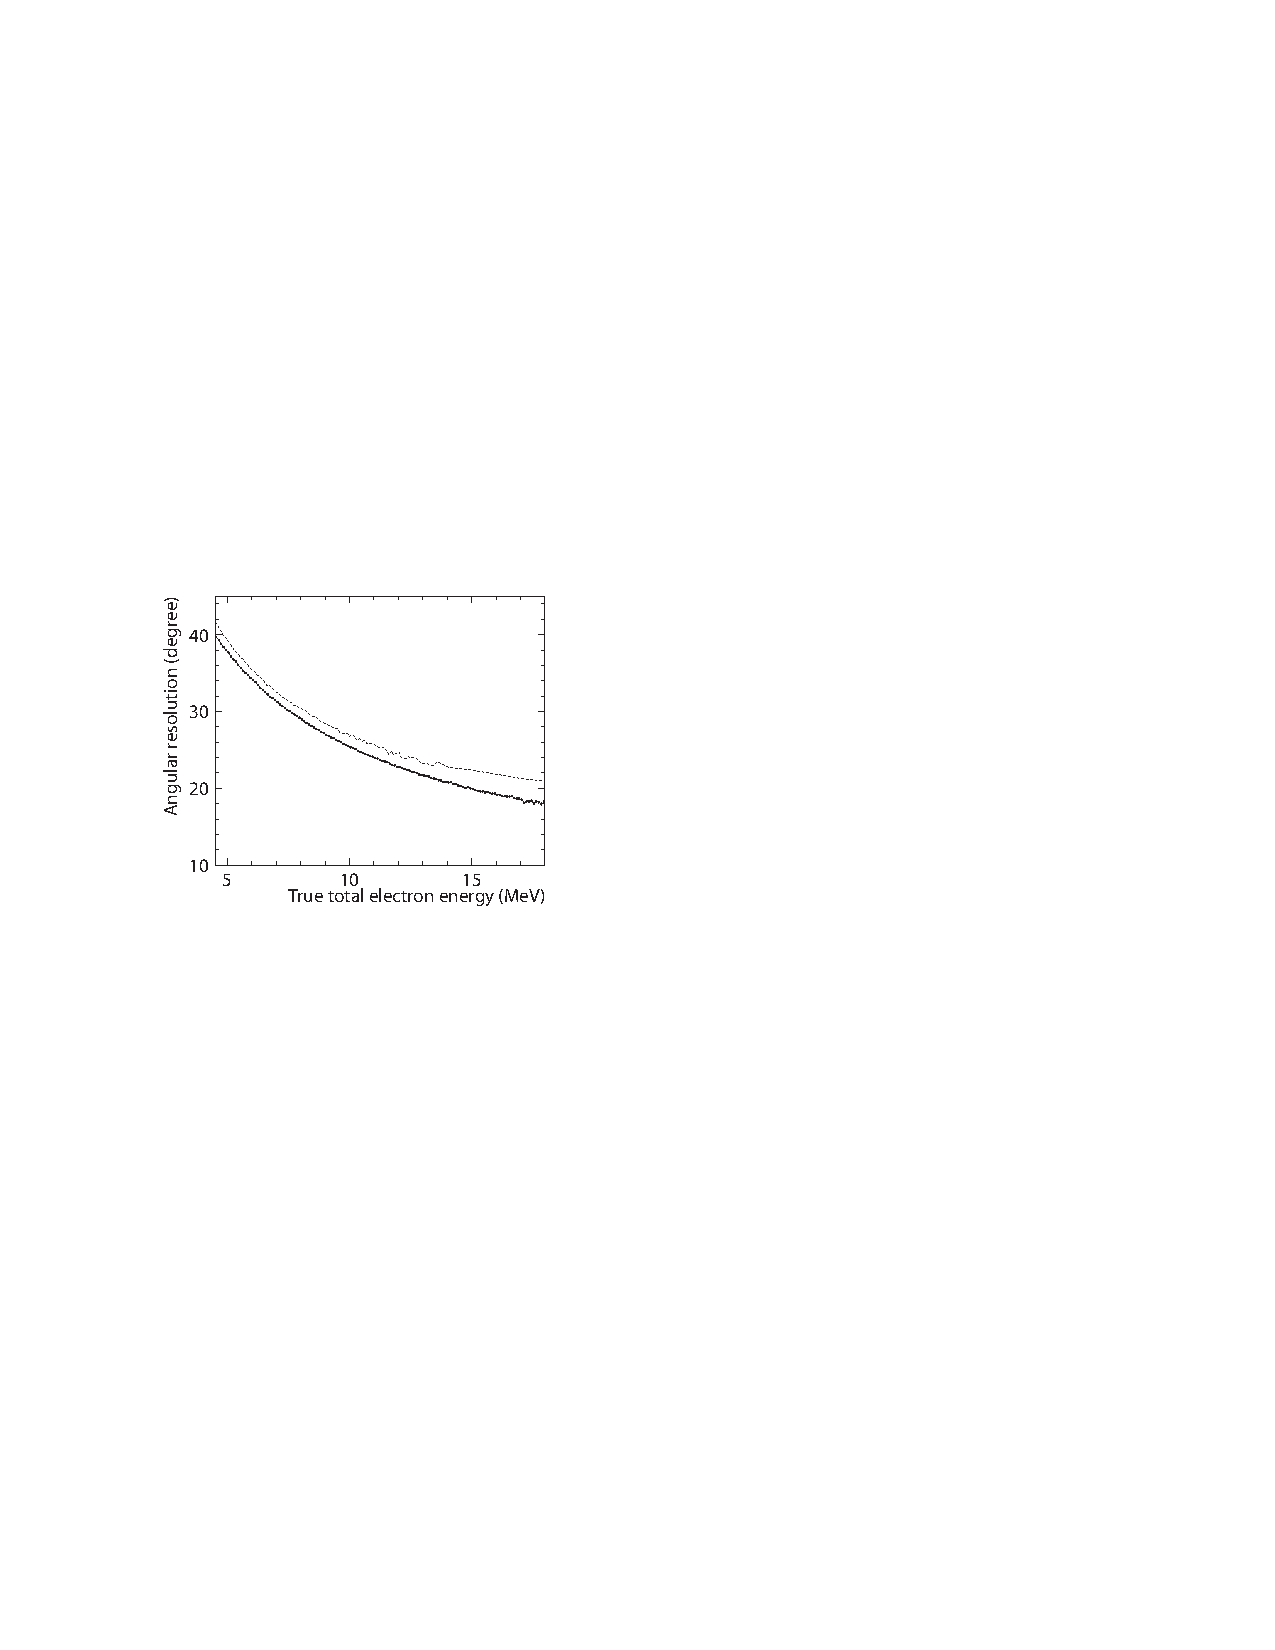
\includegraphics[width=0.8\textwidth]{reconstruction/SK-dir.pdf}}
		\caption{SK's direction resolution from SK-III~\cite{SK3}}
		\label{fig:SKdir_pos}
	\end{subfigure}%
	\caption{The relationship between resolution and energy of electrons.}
\end{figure}

